% V4 MAJOR-REVISION WORKING VERSION -- based on correccion_v3.tex.
% Track-change convention used in this file:
%   struck-through black text = only the exact previous wording being replaced
%   green text = only the exact replacement/addition; unchanged wording remains unmarked
%   red text = internal comments, missing evidence, doubts, or actions still pending
%  LaTeX support: latex@mdpi.com 
%  For support, please attach all files needed for compiling as well as the log file, and specify your operating system, LaTeX version, and LaTeX editor.

%=================================================================
\documentclass[electronics,article,submit,moreauthors]{Definitions/mdpi} 
%\documentclass[preprints,article,submit,moreauthors]{Definitions/mdpi} 
% For posting an early version of this manuscript as a preprint, you may use "preprints" as the journal. Changing "submit" to "accept" before posting will remove line numbers.

%--------------------
% Class Options:
%--------------------
%----------
% journal
%----------
% Choose between the following MDPI journals:
% accountaudit, acn, acoustics, actuators, addictions, addictprev, adhesives, adolescents, aerobiology, aerospace, agriculture, agriengineering, agrochemicals, agronomy, ai, aichem, aieng, aimater, aimed, aipa, air, aisens, aisoc, algorithms, allergies, alloys, amh, analog, analytica, analytics, anatomia, anesthres, animals, antibiotics, antibodies, antioxidants, applbiosci, appliedchem, appliedmath, appliedphys, applmech, applmicrobiol, applnano, applsci, aps, aquacj, archaeolstud, architecture, arm, arthropoda, asc, asi, astronautics, astronomy, atmosphere, atoms, audiolres, automation, axioms, bacteria, batteries, bdcc, beverages, biochem, bioengineering, biologics, biology, biomass, biomechanics, biomed, biomedicines, biomedinformatics, biomimetics, biomolecules, biophysica, bioresourbioprod, biosensors, biosphere, biotech, birds, blockchains, bloods, blsf, brainsci, breath, buildings, cancers, carbon, cardio, cardiogenetics, cardiovascmed, catalysts, cells, ceramics, challenges, chemengineering, chemistry, chemosensors, chemproc, children, chips, cimb, civileng, cleantechnol, climate, clinbioenerg, clinpract, clockssleep, cmd, cmtr, coasts, coatings, colloids, colorants, commodities, complexities, complications, compounds, computation, computers, condensedmatter, conservation, constrmater, cosmetics, covid, crops, cryo, cryptography, crystals, csmf, ctn, culture, curroncol, cyber, dairy, data, ddc, dentistry, dermato, dermatopathology, designs, devices, dhi, diabetology, diagnostics, dietetics, digital, disabilities, diseases, diversity, dna, drones, drugreact, drylands, dynamics, earth, ebj, ecm, ecologies, edm, eesp, electricity, electrochem, electronicmat, electronics, embodiedintell, encyclopedia, endocrines, energies, eng, engproc, entomology, entropy, environments, environremediat, epidemiologia, epigenomes, esa, est, fermentation, fibers, fintech, fire, fishes, fluids, foodeng, foods, forecasting, forensicsci, forests, fossstud, foundations, fractalfract, freshwater, fuels, future, futureinternet, futurepharmacol, futurephys, futuretransp, galaxies, gases, gastroent, gastrointestdisord, gastronomy, gels, genes, geochem, geographies, geohazards, geomatics, geometry, geosciences, geotechnics, geriatrics, germs, glacies, grainsci, grasses, green, greenhealth, gucdd, gynecolcancer, hardware, hazardousmatters, healthcare, healthcmater, hearts, hemato, hematolrep, hep, heritage, higheredu, highthroughput, horticulturae, hospitals, hydrobiology, hydrogen, hydrology, hydrometeorology, hydropower, hygiene, idr, iic, ijem, ijerph, ijgi, ijmd, ijms, ijns, ijom, ijp, ijpb, ijt, ijtm, ijtpp, ijtst, ime, immuno, industries, inflammj, informatics, information, infrastructures, inorganics, insects, instruments, inventions, iot, j, jaestheticmed, jal, japma, jcdd, jcm, jcp, jcrm, jcs, jcto, jdad, jdb, jdream, jemr, jeta, jfb, jfmk, jfth, jgbg, jgg, jimaging, jlpea, jmahp, jmmp, jmms, jmp, jmse, jne, jnt, jof, joi, joitmc, joma, jop, joptm, jor, jox, jpbi, jphytomed, jpm, jsan, jtaer, jvd, jzbg, kidneydial, kinasesphosphatases, knowledge, labmed, laboratories, lam, land, lasers, legumes, life, lights, limnolrev, lipidology, liquids, livers, logics, logistics, lubricants, lymphatics, machines, macromol, magnetism, magnetochemistry, make, marinedrugs, maritime, materials, materproc, mathematics, mca, mcb, measurements, medicina, medicines, medsci, membranes, merits, metabolites, metals, meteorology, methane, metrics, metrology, micro, microarrays, microbiolres, microelectronics, micromachines, microorganisms, microplastics, microwave, minerals, mining, mmphys, modelling, molbank, molecules, mollusca, mps, msf, mti, multimedia, muscles, nanoenergyadv, nanomanufacturing, nanomaterials, ncrna, ndt, network, neuroglia, neuroimaging, neurolint, neurosci, nitrogen, notspecified, nursrep, nutraceuticals, nutrients, obesities, occuphealth, oceans, ohbm, onco, optics, oral, organics, organoids, osteology, oxygen, pandemics, parasites, parasitologia, particles, pathogens, pathophysiology, pediatrrep, pets, pharmaceuticals, pharmaceutics, pharmacoepidemiology, pharmacy, phc, philosophies, photochem, photonics, photovoltaics, phycology, physchem, physics, physiologia, plants, plasma, platforms, pollutants, polymers, polysaccharides, populations, poultry, powders, precision, precisoncol, preprints, proceedings, processes, prosthesis, proteomes, psf, psychiatryint, psychoactives, purification, quantumrep, quaternary, qubs, radiation, rareearths, rdt, reactions, realestate, receptors, recycling, regeneration, remotesensing, reports, reprodmed, resources, rheumato, rjpm, robotics, rsee, ruminants, safety, sanpp, sca, sci, scipharm, sclerosis, seeds, sensors, separations, sexes, shi, signals, sinusitis, siuj, skins, smartcities, smartfish, sna, societies, software, soilsystems, solar, solids, spectroscj, sports, standards, stats, std, stratsediment, stresses, strokerep, superintelligence, surfaces, surgeries, suschem, sustainability, sustainfoods, sustainpackag, symmetry, synbio, systems, tae, targets, taxonomy, technologies, telecom, test, textiles, thalassrep, therapeutics, thermo, timespace, tomography, toxics, toxins, tph, transplantology, transportation, traumacare, traumas, tri, tropicalmed, universe, urbansci, uro, vaccines, vehicles, venereology, vetsci, vibration, virtualworlds, viruses, vision, waste, water, welding, wem, wevj, wild, wind, women, world, zoonoticdis

%---------
% article
%---------
% The default type of manuscript is "article", but can be replaced by: 
% abstract, addendum, article, benchmark, book, bookreview, briefcommunication, briefreport, casereport, changes, clinicopathologicalchallenge, comment, commentary, communication, conceptpaper, conferenceproceedings, correction, conferencereport, creative, datadescriptor, discussion, entry, expressionofconcern, extendedabstract, editorial, essay, erratum, fieldguide, hypothesis, interestingimages, letter, meetingreport, monograph, newbookreceived, obituary, opinion, proceedingpaper, projectreport, reply, retraction, review, perspective, protocol, shortnote, studyprotocol, supfile, systematicreview, technicalnote, viewpoint, guidelines, registeredreport, tutorial,  giantsinurology, urologyaroundtheworld
% supfile = supplementary materials

%----------
% submit
%----------
% The class option "submit" will be changed to "accept" by the Editorial Office when the paper is accepted. This will only make changes to the frontpage (e.g., the logo of the journal will get visible), the headings, and the copyright information. Also, line numbering will be removed. Journal info and pagination for accepted papers will also be assigned by the Editorial Office.

%------------------
% moreauthors
%------------------
% If there is only one author the class option oneauthor should be used. Otherwise use the class option moreauthors.

%=================================================================
% MDPI internal commands - do not modify
\firstpage{1} 
\makeatletter 
\setcounter{page}{\@firstpage} 
\makeatother
\pubvolume{1}
\issuenum{1}
\articlenumber{0}
\pubyear{2026}
\copyrightyear{2026}
%\externaleditor{Firstname Lastname} % More than 1 editor, please add `` and '' before the last editor name
\datereceived{ } 
\daterevised{ } % Comment out if no revised date
\dateaccepted{ } 
\datepublished{ } 
%\datecorrected{} % For corrected papers: "Corrected: XXX" date in the original paper.
%\dateretracted{} % For retracted papers: "Retracted: XXX" date in the original paper.
%\doinum{} % Used for some special journals, like molbank
%\pdfoutput=1 % Uncommented for upload to arXiv.org
%\CorrStatement{yes}  % For updates
%\longauthorlist{yes} % For many authors that exceed the left citation part
%\IsAssociation{yes} % For association journals

%=================================================================
\usepackage{listings}
\usepackage{caption}
\usepackage{subcaption}
\usepackage{tabularx}
\usepackage{booktabs}
\usepackage{makecell}
\usepackage{array}
\usepackage[normalem]{ulem}

\newcolumntype{Y}{>{\raggedright\arraybackslash}X}

% ==================== REVISION V4 MARKUP ====================
% Previous wording is struck through, replacement/additional manuscript text is green,
% and only internal comments/doubts are red.
\DeclareRobustCommand{\deleted}[1]{\textcolor{black}{\sout{#1}}}
\DeclareRobustCommand{\added}[1]{\textcolor{green!50!black}{#1}}
\DeclareRobustCommand{\changed}[2]{\deleted{#1} \added{#2}}
\newcommand{\reviewnote}[1]{\par\noindent\textcolor{red}{[#1]}\par}
% Hyperref is loaded by the MDPI class at begin-document time, so these
% PDF-string fallbacks must be registered only after hyperref is available.
\AtBeginDocument{%
  \pdfstringdefDisableCommands{%
    \def\deleted#1{}%
    \def\added#1{#1}%
    \def\changed#1#2{#2}%
    \def\reviewnote#1{}%
  }%
}
% ============================================================


\definecolor{codegreen}{rgb}{0,0.6,0}
\definecolor{codegray}{rgb}{0.5,0.5,0.5}
\definecolor{codepurple}{rgb}{0.58,0,0.82}
\definecolor{backcolour}{rgb}{0.95,0.95,0.92}
\lstdefinestyle{mystyle}{
    backgroundcolor=\color{backcolour},   
    commentstyle=\color{codegreen},
    keywordstyle=\color{magenta},
    numberstyle=\tiny\color{codegray},
    stringstyle=\color{codepurple},
    literate=
    {\{}{{{\color{black}\{}}}1
    {\}}{{{\color{black}\}}}}1
    {[}{{{\color{black}[}}}1
    {]}{{{\color{black}]}}}1
    {)}{{{\color{black})}}}1
    {(}{{{\color{black}(}}}1,
    basicstyle=\ttfamily\footnotesize,
    breakatwhitespace=false,         
    %breaklines=true,                 
    captionpos=b,                    
    keepspaces=true,                 
    numbers=left,                    
    numbersep=5pt,                  
    showspaces=false,                
    showstringspaces=false,
    showtabs=false,                  
    tabsize=2
}

\lstset{style=mystyle}

% Add packages and commands here. The following packages are loaded in our class file: fontenc, inputenc, calc, indentfirst, fancyhdr, graphicx, epstopdf, lastpage, ifthen, float, amsmath, amssymb, lineno, setspace, enumitem, mathpazo, booktabs, titlesec, etoolbox, tabto, xcolor, colortbl, soul, multirow, microtype, tikz, totcount, changepage, attrib, upgreek, array, tabularx, pbox, ragged2e, tocloft, marginnote, marginfix, enotez, amsthm, natbib, hyperref, cleveref, scrextend, url, geometry, newfloat, caption, draftwatermark, seqsplit
% cleveref: load \crefname definitions after \begin{document}


%=================================================================
% Please use the following mathematics environments: Theorem, Lemma, Corollary, Proposition, Characterization, Property, Problem, Example, ExamplesandDefinitions, Hypothesis, Remark, Definition, Notation, Assumption
%% For proofs, please use the proof environment (the amsthm package is loaded by the MDPI class).

%=================================================================
% Full title of the paper (Capitalized)
\Title{\deleted{Regulatory Compliant}\added{Regulation-Aware} Static Obstacle Avoidance Navigation Algorithm for Drone-Based Power Line Inspection}

% Author Orchid ID: enter ID or remove command
\newcommand{\orcidauthorA}{0009-0000-0483-9274} % Add \orcidA{} behind the author's name
\newcommand{\orcidauthorB}{0000-0003-2221-191X} % Add \orcidB{} behind the author's name
\newcommand{\orcidauthorC}{0000-0002-5346-2562} % Add \orcidC{} behind the author's name
\newcommand{\orcidauthorD}{0000-0002-7341-9529} % Add \orcidD{} behind the author's name

% Authors, for the paper (add full first names)
\Author{Pablo De Porcellinis $^{1,3*}$\orcidA{}, Xabier Olaz $^{2,3}$\orcidB{}, Daniel Aláez $^{2,3}$\orcidC{}, Jesus Villadangos Alonso $^{2,3}$\orcidD{}}

%\longauthorlist{yes}

% MDPI internal command: Authors, for metadata in PDF
\AuthorNames{Pablo De Porcellinis, Xabier Olaz, Daniel Aláez and Jesus Villadangos}

% Affiliations / Addresses (Add [1] after \address if there is only one affiliation.)
\address{%
$^{1}$ \quad FuVeX\\
$^{2}$ \quad Institute of Smart Cities. Universidad Pública de Navarra. 31006 Pamplona (Spain)\\
$^{3}$ Universidad Pública de Navarra}

% Contact information of the corresponding author
\corres{Correspondence: p.porcellinis@fuvex.com}

% Current address and/or shared authorship
%\firstnote{Current address: Affiliation.}  
% Current address should not be the same as any items in the Affiliation section.

%\secondnote{These authors contributed equally to this work.}
% The commands \thirdnote{} till \eighthnote{} are available for further notes.

%\simplesumm{} % Simple summary

%\conference{} % An extended version of a conference paper

% Abstract (Do not insert blank lines, i.e. \\) 
\abstract{\deleted{In an increasing world of autonomous Unmanned Aerial Vehicles}\added{Autonomous unmanned-aircraft} obstacle avoidance \deleted{solution, most of the algorithms focus on collision-free flight, geometric efficiency, or dynamic feasibility, while only limited}\added{is a mature research area, but comparatively less} work addresses \deleted{the}\added{controller-level behavior motivated by} European \deleted{regulatory logic that an autonomous route should avoid exposing protected ground parties to unnecessary overflight risk}\added{ground-risk and no-overflight considerations during an inspection mission that is already in progress}. This paper presents \deleted{Path Planning Obstacle Avoidance Regulatory Compliant Evasion}\added{PORCE}, a deterministic \deleted{real-time local replanning}\added{online local-replanning} method for waypoint-preserving obstacle avoidance in autonomous power-line inspection missions. The method \deleted{is implemented and evaluated inside a simulated environment in Unreal Engine simulator, where it operates together with}\added{integrates} a waypoint-driven flight controller, a \deleted{You-Only-Look-Once-based}\added{You Only Look Once-based} perception front-end, \deleted{and a  }monocular obstacle geopositioning\deleted{. In addition to this environment, the proposed solution is tested in a real-world scenario, where the obtained results support the transferability of the approach from simulation to real Unmanned Aerial Vehicles operation. In this implementation, civilian-like detections and nearby}\added{, and a bounded A-star local planner. Detected protected} entities are converted into \deleted{protected}\added{temporary} local \deleted{no-fly}\added{exclusion} regions\deleted{ that trigger conservative detours instead of nominal overflight. This proposed method combines European Union Aviation Safety Agency-motivated no-overflight objective with deterministic online local replanning and autonomous power-line inspection integration. The presented results show the proposed solution as a reproducible, low-overhead, and auditable local replanning method that operationalizes part}\added{; nominal navigation is preserved outside a speed-adaptive reaction horizon and temporarily inhibited when a local conflict is detected. In the logged simulation campaign, the audited encounter triggered at 60.1~m, consistent with the 61~m configured horizon at the 8~m/s cruise speed, reached a minimum logged horizontal distance of 29.6~m to the nearest perceived obstacle in the audited run, and added less than 1\% path length in the complete evasion runs. PORCE was also integrated into an experimental unmanned aircraft system and exercised in a real-world static-obstacle scenario, where flight-log evidence shows obstacle-triggered trajectory modification followed by route reattachment. These results support the feasibility and auditability} of the \deleted{European ground-risk logic at the online controller level.}\added{bounded local-replanning architecture within the demonstrated scenarios. The method is regulation-aware by design motivation, and apply some assumptions as maintain a height close to the infrastructure to remain at an Atypical Air Environment to deal with the air risk. But the present evidence does not establish formal regulatory compliance, complete Specific Operations Risk Assessment implementation, perception accuracy, comparative superiority, or measured real-time performance on the onboard hardware.}}



% Keywords
\keyword{Ground risk; \deleted{Path planning; Regulation Compliance}\added{local replanning; regulation-aware navigation}; safety-critical navigation; SORA; \deleted{UAV}\added{UAS} inspection; uninvolved people\deleted{,}\added{;} perception} 

% The fields PACS, MSC, and JEL may be left empty or commented out if not applicable
%\PACS{J0101}
%\MSC{}
%\JEL{}

%%%%%%%%%%%%%%%%%%%%%%%%%%%%%%%%%%%%%%%%%%
% Only for the journal Diversity
%\LSID{\url{http://}}

%%%%%%%%%%%%%%%%%%%%%%%%%%%%%%%%%%%%%%%%%%
% Only for the journal Applied Sciences
%\featuredapplication{Authors are encouraged to provide a concise description of the specific application or a potential application of the work. This section is not mandatory.}
%%%%%%%%%%%%%%%%%%%%%%%%%%%%%%%%%%%%%%%%%%

%%%%%%%%%%%%%%%%%%%%%%%%%%%%%%%%%%%%%%%%%%
% Only for the journal Data
%\dataset{DOI number or link to the deposited data set if the data set is published separately. If the data set shall be published as a supplement to this paper, this field will be filled by the journal editors. In this case, please submit the data set as a supplement.}
%\datasetlicense{License under which the data set is made available (CC0, CC-BY, CC-BY-SA, CC-BY-NC, etc.)}

%%%%%%%%%%%%%%%%%%%%%%%%%%%%%%%%%%%%%%%%%%
% Only for the journal BioTech, Fishes, Neuroimaging and Toxins
%\keycontribution{The breakthroughs or highlights of the manuscript. Authors can write one or two sentences to describe the most important part of the paper.}

%%%%%%%%%%%%%%%%%%%%%%%%%%%%%%%%%%%%%%%%%%
% Only for the journal Encyclopedia
%\encyclopediadef{For entry manuscripts only: please provide a brief overview of the entry title instead of an abstract.}

%%%%%%%%%%%%%%%%%%%%%%%%%%%%%%%%%%%%%%%%%%
% Different journals have different requirements. Please check the specific journal guidelines in the "Instructions for Authors" on the journal's official website.
%\addhighlights{yes}
%\renewcommand{\addhighlights}{%
%
%\noindent This is an optional section, the goal of which is to increase the discoverability and readability of the article via search engines and other scholars. Highlights should not be a copy of the abstract, but a simple overview allowing the reader to quickly and simply find out what the article is about and what can be cited from it. Each of these parts should be up to 2 bullet points.\vspace{3pt}\\
%\textbf{What are the main findings?}
% \begin{itemize}[labelsep=2.5mm,topsep=-3pt]
% \item First bullet.
% \item Second bullet.
% \end{itemize}\vspace{3pt}
%\textbf{What are the implications of the main findings?}
% \begin{itemize}[labelsep=2.5mm,topsep=-3pt]
% \item First bullet.
% \item Second bullet.
% \end{itemize}
%}

%%%%%%%%%%%%%%%%%%%%%%%%%%%%%%%%%%%%%%%%%%
\begin{document}

\reviewnote{REVISION DEL ABSTRACT: Hay que revisar esta frase:"But the present evidence does not establish formal regulatory compliance, complete Specific Operations Risk Assessment implementation, perception accuracy, comparative superiority, or measured real-time performance on the onboard hardware" porque quizás es "atacar" directamente en el abstract a nuestro propio método. Igual en limitations al final tiene todo el sentido, pero no se si en el abstract puede jugar en nuestra contra.}
\reviewnote{REVISION DEL ABSTRACT: Hay que tener en cuenta que en las normas se supone que el abstract está limitado en "about 200 words maximum"}

\reviewnote{Aqu\'i hemos cambiado el t\'itulo a ``Regulation-Aware'' porque con los datos actuales no demostramos cumplimiento regulatorio formal. Si por continuidad del nombre o por una decisi\'on editorial necesitamos conservar ``Regulatory Compliant'', tenemos que decidirlo antes de enviar y explicar expresamente que no estamos reclamando aprobaci\'on SORA completa (R4-D9).}
\reviewnote{Aqu\'i nos siguen faltando las cifras de la campa\~na real para cerrar del todo el abstract: cu\'antos vuelos hicimos, cu\'antos salieron bien/mal, clearance m\'inimo, longitud y duraci\'on, tiempo de replanning y consumo si se registr\'o. No metemos ning\'un n\'umero hasta sacarlo de los logs (R1-1, R4-A4).}

%%%%%%%%%%%%%%%%%%%%%%%%%%%%%%%%%%%%%%%%%%
\section{Introduction}

Unmanned Aerial Vehicles (UAVs) are becoming a practical tool for infrastructure inspection, surveillance, and monitoring, with a growing impact in agriculture, critical infrastructure, and other industrial environments \cite{imran2025environmental,marut2024surveillance}. Power-line inspection constitutes a particularly relevant use case, as it combines long-range navigation, repetitive geometric structures, constrained mission corridors, and the need to react to unforeseen obstacles while maintaining the inspection objectives. The operational experience of companies such as FuVeX has revealed several technological and methodological challenges that remain to be addressed, while also highlighting the importance of simulation-based development. 

Testing navigation strategies in representative simulated environments enables systematic assessment under controlled and repeatable conditions, contributes to risk reduction, and facilitates the application of insights gained through simulation to subsequent field operations. Simulation should therefore not be regarded merely as a preliminary verification stage, but rather as an integral component of the design, integration, and maturation of autonomous guidance solutions. This perspective motivates the simulation-oriented methodology adopted in this work.

From a planning point of view, the \deleted{Powerline Inspection}\added{power-line inspection} scenario is \deleted{difficult}\added{challenging} because the vehicle must maintain a global mission structure while responding online to local conflicts. Purely global planners are efficient when the environment is static and fully known, but their performance may degrade under late obstacle appearance or perception uncertainty \cite{debnath2024review,meng2025advances}. On the other hand, fully learned end-to-end policies are harder to audit in safety-critical aeronautical contexts, where traceability and bounded behavior remain important design properties \cite{EASA_AI_Roadmap_2.0}.

The regulatory dimension makes the problem even sharper. Under the UAS regulatory framework of the European Union, the operational core was defined by the Commission Implementing Regulation (EU) 2019/947 on the rules and procedures for the operation of unmanned aircraft and the Commission Delegated Regulation (EU) 2019/945 on unmanned aircraft systems, while, more recently, EASA AMC/GM material now incorporates the JARUS SORA 2.5 package for the `specific' category \cite{EU2019_947,EU2019_945,JARUS_SORA_2_5_2024,EASA_AMC_GM_SORA25_2025}. Within this framework, the acceptability of a route is not only a matter of geometric collision avoidance but also of limiting exposure of uninvolved people and sensitive ground areas. This means that an autonomous planner should not simply ask whether the UAV \emph{can} fly over a location, but whether it \emph{should} do so in a risk-aware operational sense. The existing literature has already started to encode this concern through urban risk maps, third-party risk models, SORA-aware cost functions, and target-level-of-safety constraints \cite{primatesta2019riskaware,primatesta2020groundrisk,pang2022integrated,tang2023thirdparty,zhang2023groundrisk,heinze2023sora,brassel2025riskaware}. However, most of these works remain strategic route optimizers or city-scale risk planners rather than controller-level local replanners for infrastructure inspection missions already in progress.

 The present paper does not claim to encode the full legal tables of open-category separation or the full SORA mitigation calculus within the planner. Instead, it implements the narrower controller-level step that those regulatory mechanisms motivate: live civilian-like detections are converted into temporary protected regions that the UAV should avoid crossing.

\deleted{This paper focuses on Path Planning and Obstacle Avoidance Regulatory Compliant Evasion (PORCE) as the main scientific contribution. Its role is simple but operationally important: whenever an obstacle enters a conservative reaction horizon, the method temporarily inhibits nominal navigation, computes a}\added{PORCE is not presented as a new object detector or as a new shortest-path algorithm. Its contribution is the controller-level integration rule that links live georeferenced detections, temporary protected regions, a speed-adaptive activation condition,} bounded local \deleted{path}\added{A* replanning} toward the \deleted{current}\added{active} mission waypoint, \deleted{and returns control}\added{explicit failsafe escalation, and automatic reattachment} to the \deleted{original}\added{nominal inspection} route\deleted{ as soon as}\added{. This combination makes} the local \deleted{conflict disappears. The novelty}\added{avoidance action bounded and auditable while preserving the semantics of the pre-planned mission. The scientific claim} is therefore \deleted{not obstacle avoidance in isolation. The novelty is to operationalize a regulatory-aware no-overflight logic for uninvolved third parties and nearby protected entities inside a deterministic, online local replanner. The work is therefore intentionally framed within this EASA-relevant operational niche, where the proposed method advances the state of the art}\added{deliberately narrow: PORCE addresses detection-driven, ground-risk-motivated local replanning during an inspection mission already in progress}, rather than \deleted{as a universal solution intended to supersede existing approaches to }generic \deleted{UAV}\added{obstacle} avoidance or \added{strategic }risk-aware route \deleted{planning.}\added{optimization.}

The main contributions of this paper are the following.
\begin{itemize}
    \item \deleted{The definition}\added{The proposal} of PORCE as a deterministic, waypoint-preserving local replanning \deleted{method for real-time UAV obstacle}\added{architecture that converts detected protected entities into hard local exclusion regions and activates bounded} avoidance \deleted{in power-line}\added{without redefining the global} inspection \deleted{missions, explicitly motivated by European ground-risk and no-overflight concerns.}\added{mission.}
    \item \deleted{A formal and reproducible description of how the method is}\added{The formalization and implementation of the complete controller chain: speed-adaptive triggering, class-dependent obstacle inflation, bounded $81\times81$ A* search with 6~m cells, route reattachment, and failsafe escalation,} integrated with perception\deleted{, Mission execution, and evaluation of results inside a validated simulation environment.}\added{ and mission execution.}
    \item \deleted{Real-world scenario tests, where the results obtained support the transferability}\added{Quantitative evaluation} of the \deleted{approach from}\added{static-obstacle behavior in} simulation \deleted{to real UAV operation.}\added{together with physical-UAS integration and field execution. In the audited simulation encounter, the first replan occurs at 60.1~m for a 61~m configured horizon, the minimum logged distance to the nearest perceived obstacle is 29.6~m, and complete evasion missions add less than 1\% to the obstacle-free mission path; the field campaign provides evidence of onboard detection, evasion, and route reattachment but is not yet supported by the same aggregate metric set.}
\end{itemize}

\added{The remainder of the paper is organized as follows. Section~2 reviews related work on UAV navigation, power-line inspection, ground-risk-aware planning, landing, and local obstacle avoidance. Section~3 summarizes the regulatory and technical background used to motivate the controller design. Section~4 formalizes the PORCE method and its bounded replanning logic. Section~5 describes the simulation and real-world experimental setups. Section~6 reports the simulation and field results. Section~7 states the limitations of the current evidence, and Section~8 summarizes the conclusions and future validation work.}


\section{Related Works}
% No está claro si la combinación en la sección de related works es sin subtítulos o no. Creo que queda un popurri si no se separan las secciones aunque creemos esta nueva. 
%\subsection{State of the Art}
Vision-based UAV navigation has been widely studied as a perception-driven alternative to map-only planning, with applications ranging from localization to obstacle detection and local trajectory generation. These techniques are often motivated by scenarios where Global Navigation Satellite Systems (GNSS) signals are unavailable, unreliable, or degraded, although their applicability is not limited to such conditions \cite{arafat2023vision,huang2025investigation}. Recent reviews classify UAV-path planning and obstacle-avoidance approaches according to different criteria, including the representation of the environment, the planning strategy, and the information available during flight \cite{debnath2024review, merei2025survey, meng2025advances}.

2D formulations represent the operating environment on a plane, commonly through occupancy, grid or cost maps \cite{merei2025survey}. Deterministic graph-search methods such as Dijkstra and A* can be applied when the environment is represented as a graph or discretized search space \cite{lavalle2006planning}.

3D formulations extend the planning space by incorporating altitude variations and volumetric obstacle representations. This allows the planner to exploit both horizontal and vertical maneuvers, at the cost of a larger search space and, depending on the application, additional kinematic  or dynamic constraints \cite{merei2025survey, nafees2026review}. The distinction between 2D and 3D planning therefore concerns representation of the navigation problem rather than the use of a particular planning algorithm. Graph-search, sampling-based, optimization-based, and hybrid methods can be formulated for different state space representations depending on the mission requirements \cite{lavalle2006planning, meng2025advances}.

Another relevant question concerns when the trajectory is generated. Global planning methods generally plan from environmental information available before execution, whereas local planning and replanning approaches modify the trajectory during flight as new information becomes available \cite{debnath2024review, meng2025advances}. Related spatial constraints can also be introduced through geofencing, where keep-in or keep-out regions are explicitly incorporated into the planning or traffic-management process \cite{stevens2021geofence}.

In power-line inspection, several works have addressed the perception and reconstruction of the surrounding environment. These include an image-based inspection method that estimates the spatial position of powerlines, reconstructs dense point clouds of the corridor \cite{zhang2017powerline}, a Lidar-supported automatic inspection and collision-free route generation \cite{guan2021uavlidar}, and dual-view stereovision for the reconstruction of three-dimensional corridors \cite{zhou2022dualview}. Deep learning approaches have also been applied to \deleted{ral-time}\added{real-time} infrastructure detection \cite{bellou2024aerial}, while recent reviewers summarize the increasing role of autonomous perception in this field \cite{mendu2025state, faisal2025deep}.

Path planning has also been specifically considered for UAV-based power-line inspection. Huang \emph{et al.} \deleted{purposes and}\added{propose a} hybrid approach that combines an improved \deleted{RTT*}\added{RRT*} for global path planning with DWA for local obstacle avoidance \cite{huang2025hybrid}. Their work focuses on collision avoidance and trajectory optimization in inspection scenarios, providing an example of how global and local planning strategies can be combined for UAV-based power inspection. 

Beyond conventional collision avoidance and trajectory adaptation, UAV inspection missions may also be constrained by the ground risk approach. This aspect introduces a different set of operational considerations, directly related to regulatory concerns. 

%PARRAFOS ANTUGUOS: 
% Vision-based UAV navigation has been widely studied as a perception-driven alternative to map-only planning, with applications ranging from localization to obstacle detection and local trajectory generation. Although these techniques are often motivated by scenarios where Global Navigation Satellite Systems (GNSS) signals are unavailable, unreliable, or degraded, the literature has demonstrated that vision-based approaches are not limited to such conditions \cite{arafat2023vision,huang2025investigation}.

%However, there are general reviews of UAV navigation that integrate this type of techniques and consistently distinguish between global and local path planning paradigms. Global path planning methods assume a sufficiently known environment and compute a static solution in advance based on prior maps or predefined constraints. Classical search algorithms such as Dijkstra or A* have been employed within this paradigm and can perform effectively in fully mapped and static environments \cite{lavalle2006planning}.However, their use as stand-alone solutions without integration with complementary perceptual or reactive components presents significant limitations in real-world missions such as power-line inspection or infrastructure monitoring. In contrast, local path planning approaches generate or adapt trajectories online while the vehicle is moving, allowing immediate reactions to newly perceived environmental elements encountered during flight \cite{debnath2024review,meng2025advances}. More specifically, recent surveys in 2025 and 2026 confirm that the dominant design goals remain collision avoidance, dynamic feasibility, and computational efficiency, while explicit treatment of ground exposure of third-parties is still comparatively rare in runtime planning \cite{merei2025survey,nafees2026review}. The proposed method is explicitly positioned in the online local-replanning class.

%A related runtime mechanism is dynamic geofencing, where keep-in and keep-out volumes are inserted into the planner or the traffic-management layer to organize low-altitude operations \cite{stevens2021geofence}. Geofences are, however, pre-declared or externally managed volumes: they are defined before the flight, or independently of what the aircraft currently perceives. The protected regions studied here differ in that they are generated online from live detections and remain anchored to the active mission waypoint, so the global inspection mission is temporarily inhibited rather than replaced.

%For power-line inspection, the local planning problem is more operational than academic. The vehicle must continue progressing through a mission corridor, while structures, animals, vehicles, or uninvolved people may appear in the neighborhood of the route. Power-line inspection has therefore developed its own system literature, from UAV-image approaches for corridor measurement and obstacle localization \cite{zhang2017powerline} to line detection in cluttered scenes \cite{zhang2019powerlines}, LiDAR-supported automatic inspection \cite{guan2021uavlidar}, dual-view stereovision for reconstruction and clearance estimation \cite{zhou2022dualview}, and dedicated reviews of UAV-enabled power-line inspection \cite{mendu2025state}. On the perception side, Bellou \emph{et al.} report aerial inspection based on YOLOv8 for towers, conductors and insulators \cite{bellou2024aerial}, while Faisal \emph{et al.} synthesize more than 70 studies and identify persistent gaps in multimodal fusion and deployment realism \cite{faisal2025deep}. On the planning side, Huang \emph{et al.} propose a hybrid RRT*+DWA method for dynamic obstacle avoidance in UAV-based power inspection \cite{huang2025hybrid}. These works are highly relevant, but their central objective is still efficient and safe inspection autonomy, not explicit no-overflight treatment of uninvolved people under European operational logic.


A separate strand of literature addresses these regulatory and ground-risk considerations in UAS path planning. Primatesta \emph{et al.} propose a risk-aware urban path-planning strategy with off-line and on-line phases driven by risk maps \cite{primatesta2019riskaware}, and later formalized the construction of ground-risk maps for urban UAV operations \cite{primatesta2020groundrisk}. Pang \emph{et al.} incorporated third-party risks into a metropolitan cost model \cite{pang2022integrated}, while Tang \emph{et al.} considered obstacle risk, fatality risk, and property loss risk in a Min-cost A* framework \cite{tang2023thirdparty}. Pilko \emph{et al.} and Zhu \emph{et al.} further studied spatiotemporal and grid-based ground-risk mapping \cite{pilko2023spatiotemporal,zhang2023groundrisk}. More \deleted{recently}\added{recent} work by Heinze and Uijt de Haag \added{and by }Bra{\ss}el \emph{et al.} incorporates SORA and \deleted{TLS}\added{target-level-of-safety} concepts into route optimization, bringing these approaches closer to current European operational requirements\added{ }\cite{heinze2023sora,brassel2025riskaware}.\added{ }Du \emph{et al.} provide a review\added{ of} safety-risk modeling for civil UAS operations, highlighting the importance of assessment\added{-} and authorization-oriented risk \deleted{modeling}\added{models} \cite{du2024safetyrisk}.

The works discussed \deleted{avobe}\added{above} address complementary aspects of UAV navigation, including perception, obstacle \deleted{avoidande}\added{avoidance}, geofencing, ground-risk \deleted{assesment}\added{assessment} and regulatory-aware planning. The following Table \ref{tab:related_work_comparison} summarizes the main characteristics of representative approaches and compares them with the proposed method. 

\begin{table*}[t]
\caption{Comparison of representative approaches related to UAV obstacle avoidance, power-line inspection, \added{landing, }ground-risk-aware path planning, and the proposed PORCE method.}
\label{tab:related_work_comparison}

\centering
\fontsize{7.2}{8.2}\selectfont
\setlength{\tabcolsep}{1.2pt}
\renewcommand{\arraystretch}{1.12}

\begin{tabularx}{\linewidth}{
>{\raggedright\arraybackslash}p{1.05cm}
>{\raggedright\arraybackslash}p{1.20cm}
>{\centering\arraybackslash}p{1.10cm}
>{\raggedright\arraybackslash}X
>{\raggedright\arraybackslash}X
>{\centering\arraybackslash}p{0.52cm}
>{\centering\arraybackslash}p{0.48cm}
>{\centering\arraybackslash}p{0.48cm}
>{\raggedright\arraybackslash}X
>{\raggedright\arraybackslash}X
}

\toprule

\textbf{Work} &
\shortstack{\textbf{Obstacle /}\\\textbf{target type}} &
\shortstack{\textbf{Environment}\\\textbf{model}} &
\shortstack{\textbf{Detection /}\\\textbf{risk information}} &
\shortstack{\textbf{Local planning}\\\textbf{method}} &
\added{\textbf{Land.}} &
\textbf{Sim.} &
\textbf{Real} &
\shortstack{\textbf{Performance}\\\textbf{metrics}} &
\shortstack{\textbf{Uninvolved-person /}\\\textbf{no-overflight}} \\

\midrule

Zhou et al. \cite{zhou2022dualview} &
Power lines and ground objects &
3D corridor &
Dual-view stereovision, line detection, and ground-object perception &
Flight-point generation and line following; no dedicated local obstacle replanner &
\added{No} &
No &
Yes &
Ground-clearance error and processing time &
No \\

\addlinespace[2pt]

Huang et al. \cite{huang2025hybrid} &
Static and dynamic geometric obstacles &
Planar / 2D &
Map-based obstacle representation; no onboard detector evaluated &
Improved DWA local avoidance with improved RRT* global planning &
\added{No} &
Yes &
No &
Path length, node count, and planning time &
No \\

\addlinespace[2pt]

Stevens and Atkins \cite{stevens2021geofence} &
Airspace and geofence conflicts &
3D + time &
Explicitly defined UTM geofences &
Spatial and temporal geofence deconfliction; no onboard local obstacle planner &
\added{No} &
Case study &
No &
Deconfliction feasibility and impact on planned flight &
Generic keep-out regions; not person-specific or perception-triggered \\

\addlinespace[2pt]

Primatesta et al. \cite{primatesta2019riskaware} &
Population ground risk and dynamic risk factors &
2D risk map &
Static and dynamic risk maps &
riskA* offline planning and Borderland online path repair &
\added{No} &
Yes &
No &
Risk cost, computation, and path adaptation &
Ground-population risk minimization; no explicit detected-person no-overflight region \\

\addlinespace[2pt]

Pang et al. \cite{pang2022integrated} &
Fatality, property, and noise risks to third parties &
3D risk-cost environment &
Population, traffic, and risk models &
EDA-CostA* risk-aware path optimization &
\added{No} &
Yes &
No &
Risk-cost reduction &
Third-party risk incorporated into route cost; not perception-triggered \\

\addlinespace[2pt]

Tang et al. \cite{tang2023thirdparty} &
Obstacle, fatality, and property-loss risks &
3D urban risk model &
Model-based urban risk assessment &
Min-cost A* with path smoothing &
\added{No} &
Yes &
No &
Integrated risk cost and path smoothness &
Third-party risk represented through path cost; no explicit detected-person no-overflight region \\

\addlinespace[2pt]

Heinze and Uijt de Haag \cite{heinze2023sora} &
Population and infrastructure ground exposure &
3D, mainly horizontal routing &
Population and infrastructure geodata &
T-RRT* risk-based route optimization &
\added{No} &
Case study &
No &
Population exposure, path cost, and computational performance &
SORA-oriented ground-risk mitigation; not triggered by onboard person detection \\

\addlinespace[2pt]

Bra{\ss}el et al. \cite{brassel2025riskaware} &
Pedestrian and vehicle ground risk &
GIS-based ground-risk representation &
Urban GIS, exposure, and UAV risk models &
Risk-weighted A* route optimization &
\added{No} &
Yes &
No &
Ground-risk reduction, detour factor, and TLS compliance &
TLS-constrained ground-risk planning; not person-specific onboard detection \\

\addlinespace[2pt]

\added{Merei et al. \cite{merei2025esls}} &
\added{Static and dynamic obstacles during emergency descent} &
\added{3D RGB-D / point-cloud environment} &
\added{YOLOv5, RGB-D, VIO, and RTAB-MAP} &
\added{Safe-landing-zone selection and 3D obstacle-aware descent} &
\added{Yes} &
\added{Yes} &
\added{No} &
\added{Landing-zone detection accuracy, processing time, and landing success} &
\added{Survivor-aware landing; not a mission-route no-overflight replanner} \\

\addlinespace[2pt]

\textbf{PORCE (proposed)} &
\textbf{Detected static obstacles and uninvolved people} &
\textbf{2D local model} &
\textbf{YOLO-based onboard detection and monocular geopositioning} &
\textbf{Deterministic A*-based online local replanning preserving the active mission waypoint} &
\added{\textbf{No}} &
\textbf{Yes} &
\textbf{Yes} &
\deleted{\textbf{Replanning time and trajectory/avoidance performance; simulation--flight consistency}}\added{\textbf{Simulation path length, evasion duration, perceived-obstacle clearance, and replan count; field trajectory evidence}} &
\deleted{\textbf{Yes; onboard detection generates a temporary local protected no-overflight region}}\added{\textbf{Detection-triggered protected-region logic; formal regulatory compliance is not demonstrated}} \\

\bottomrule
\end{tabularx}

\vspace{1mm}

\begin{flushleft}
\fontsize{7.2}{8.2}\selectfont
``Real'' refers to validation involving a physical UAV or field operation;
the use of real-world GIS data, point clouds, or recorded imagery alone is not
classified as real-flight validation. The no-overflight column distinguishes
explicit keep-out or protected-region constraints from approaches that reduce
third-party exposure through a risk-cost function. \added{``Land.'' indicates whether the method explicitly plans or controls a landing/descent trajectory.}
\end{flushleft}

\end{table*}

\added{Emergency-landing work is related but addresses a different operational phase. ESLS uses RGB-D sensing, visual-inertial odometry, RTAB-MAP, YOLOv5, and 3D obstacle-aware descent to identify and reach a safe landing area. This is useful as a reference for 3D static/dynamic obstacle handling and landing, whereas PORCE operates during the inspection leg, preserves the current mission waypoint, and returns the vehicle to the nominal inspection route rather than selecting a landing site \cite{merei2025esls}.}

\added{Learning-based planning provides a complementary design point. Sonny \emph{et al.} evaluate a grid-graph Q-learning approach for UAV path planning with static and dynamic obstacle avoidance and compare it with A*, Dijkstra, and SARSA using path length and learning time \cite{sonny2023qlearning}. More broadly, reinforcement-learning planners can adapt navigation policies through learned rewards, but their evaluation depends on the training distribution, reward definition, convergence, and generalization assumptions \cite{meng2025advances}. PORCE deliberately retains deterministic graph search so that its online decision chain and failure modes remain explicit during safety-oriented validation; this is a design trade-off, not a claim that deterministic planning is universally superior.}

\reviewnote{Aqu\'i nos sigue faltando la comparaci\'on cuantitativa en el mismo escenario contra un A* local sin la l\'ogica PORCE, RRT*, DWA y los otros baselines que pide el revisor. Para comparar longitud, tiempo de c\'omputo y clearance de forma seria tenemos que ejecutar todos con el mismo mapa, velocidad, obst\'aculos y criterio de \'exito. Si no tenemos esas ejecuciones, lo dejamos como limitaci\'on y no inventamos una tabla de resultados (R3-3, R1-5, R4-D8).}
\reviewnote{La discusi\'on de reinforcement learning ya la podemos cubrir a nivel bibliogr\'afico. Lo que no tenemos es un benchmark experimental PORCE vs. Q-learning/DRL, as\'i que no debemos vender una comparaci\'on de rendimiento que no hemos ejecutado (R3-7).}
\reviewnote{Con ``EAODA'' seguimos teniendo una duda concreta: con ese acr\'onimo no hemos podido identificar de forma inequ\'ivoca el art\'iculo al que se refiere el revisor. Nos hace falta el t\'itulo o DOI exacto para no citar el trabajo equivocado. En cuanto lo tengamos, metemos la fila y la comparaci\'on bibliogr\'afica al lado de ESLS.}



\paragraph{Research gap.}
Existing work has addressed both ground-risk considerations and risk-aware path planning for UAV operations. However, these approaches generally optimize geometric avoidance without an explicit uninvolved-people objective, or address ground risk at a strategic route-planning level rather than during the online execution of an inspection mission. Less attention has been given to the local guidance response required when onboard detections indicate that the nominal trajectory may overfly or pass close to an uninvolved person. 

The proposed method addresses this operational problem by converting nearby detections into protected local no-fly regions, preserving the active mission waypoint as an input for the avoidance maneuver, and reporting the resulting guidance decisions through the same telemetry. 


\section{\texorpdfstring{\added{Regulatory and Technical Background}}{Regulatory and Technical Background}}
\label{sec:regulatory_background}

\deleted{To better understand the potentiality of the proposed solution, it is necessary to explain the UAS framework}\added{The regulatory background relevant to PORCE is} defined by Regulations (EU) 2019/947 and 2019/945 and \deleted{operationalized through}\added{by the} AMC/GM \deleted{plus}\added{material that incorporates} SORA 2.5\added{ for specific-category operations} \cite{EU2019_947,EU2019_945,JARUS_SORA_2_5_2024,EASA_AMC_GM_SORA25_2025}. The key \deleted{concept around regulation is}\added{point for this work is that} operational \deleted{risk, so there are topics within this framework that transform navigation into an optimization problem with hard restrictions. The concept of an uninvolved person plays an significant role in the segmentation of categories. EASA defines it}\added{acceptability is not purely geometric: the presence of uninvolved people can introduce ground-risk constraints that affect where the aircraft should fly. PORCE uses this principle only} as a \deleted{person who}\added{controller-level motivation for avoiding detected protected entities; it} does not \deleted{participate in the UAS operation or who is not aware of the instructions and safety precautions given to the UAS operator. In contrast to a power-line tower or cable, an "uninvolved person" generates a risk field in the surrounding space that adds new constraints inside the route planning, so that route geometry cannot be judged independently from who may be under the aircraft and under what conditions.}\added{reproduce the complete regulatory assessment.}

\deleted{The concept of uninvolved people remains a central regulatory objective as risk levels increase and the operational category changes. However, it is addressed through the definition and control}\added{Within SORA, ground-risk treatment depends on the characteristics of the operation and aircraft, including parameters related to impact energy and operating height \cite{JARUS_SORA_2_5_2024}. This creates a planning trade-off: increasing speed can improve mission time, but it also changes the physical consequences} of a \deleted{Ground Risk Buffer, understood as a spatial margin surrounding the Operational Volume. The Ground Risk Buffer is therefore managed through a combination of}\added{potential ground impact. Therefore, mission-time optimization and ground-risk constraints should not be treated as independent design objectives. PORCE does not calculate the SORA ground-risk buffer online; its speed-adaptive trigger is instead a conservative controller parameterization whose quantitative mapping to an approved} operational \deleted{constraints, technical mitigation, and procedural measures, forming an integral element of the overall safety margin that must be taken into account from the path planning perspective. Within this Ground Risk Buffer definition, the Kinetic Energy ($v, m$) and height ($h$) of the UAS represent important limitation parameters. The actual path-planning algorithms optimize the velocity to reduce the mission time ($J{tiempo}$). However, as the velocity increases, the UAS expands the Ground Risk Buffer, according to the formulas of SORA Annex F \cite{JARUS_SORA_2_5_2024}. A standard planner from the literature will accelerate the improvement of efficiency \cite{dong2017efficient}, inadvertently violating the legally required safety margin.}\added{buffer remains to be demonstrated.}

\deleted{This }SORA 2.5 \deleted{methodology presented by JARUS establishes a set of ground risk mitigation factors that can be applied to reduce the ground risk level of}\added{includes ground-risk mitigations whose applicability and credit depend on} the operation \deleted{before flight. This reduction in ground risk level is crucial, as it will imply a reduction in the intrinsic risk of a person being stuck by an UA and a reduction in the level of risk of the whole operation and will allow the aircraft to fly over the expected area without the need to pass a certification process. Inside these strategic mitigations, the 'M1 (C) mitigation-Ground observation' is directly related with the concept of 'uninvolved people'. This mitigation implies that the UAS crew or the systems inside the aircraft itself can observe most}\added{and on the evidence provided by the operator. The M1(C) ground-observation mitigation is particularly relevant to the motivation of this work because it considers observation} of the overflown area\deleted{, allowing the detection of 'uninvolved people' in the operational area and maneuvering the UA so that the 'uninvolved people' are not overflown \cite{EASA_AMC_GM_SORA25_2025}.}\added{ and operational action intended to avoid overflight of uninvolved people \cite{EASA_AMC_GM_SORA25_2025}. PORCE implements only the detection-to-maneuver behavior that is conceptually aligned with this objective; whether a particular operation can claim M1(C) credit requires separate evidence and assessment.}

 The present method does not implement the full legal machinery of either level of risk. What it does implement is the controller-level behavior that every level of risk mentioned motivates: when live perception suggests that the current local corridor should not be overflown, the UAV performs a temporary local bypass instead of persisting on the nominal line.

\begin{table}[h!]
\captionsetup{justification=centering}
\caption{Traceability between the implemented controller behaviors and the regulatory provisions that motivate them. 
}
\label{tab:traceability}
\centering
\small
\begin{tabular}{@{}p{0.29\columnwidth} p{0.31\columnwidth} p{0.31\columnwidth} @{}}
\toprule
\textbf{Controller behavior} & \textbf{Motivating provision} & \added{\textbf{Still needed for formal compliance credit}} \\
\midrule
Detections converted into protected local regions with hard exclusion radii & No-overflight logic for uninvolved people (Reg.\ (EU) 2019/947; SORA ground-risk model) & \added{Class-dependent envelopes sized and validated against the applicable ground-risk model.} \\

Speed-adaptive reaction horizon & \deleted{Ground risk}\added{SORA ground-risk treatment and operational-volume/ground-risk-buffer concepts motivate conservative margins, but the PORCE horizon is not derived from the SORA} buffer \deleted{sized from impact energy and operating height (SORA Main Body Step \#2 \cite{JARUS_SORA_2_5_2024}; Annex F energy }model \deleted{\cite{JARUS_SORA_2_5_AnnexF_2024})}\added{\cite{JARUS_SORA_2_5_2024,JARUS_SORA_2_5_AnnexF_2024}.} & \added{Measured mapping between sensor range, end-to-end latency, navigation/execution error, maneuver capability, speed, and the margin required by the specific operation.} \\

Online observation of the overflown area with maneuver to avoid overflight & M1(C) ground-observation mitigation & \added{Evidence that the sensor geometry and operating concept satisfy the observation/integrity conditions required for credit.} \\

Deterministic, auditable decision chain with failsafe escalation & Traceability expectations for safety-critical functions (SORA Operational Safety Objectives (OSOs); EASA AI Roadmap) & \added{Runtime-assurance and failure-case evidence on representative onboard hardware.} \\

\bottomrule
\end{tabular}
\end{table}
 
\added{From a local-planning perspective, deterministic graph search provides a transparent basis for the bounded replanning stage because the search objective, obstacle representation, and failure condition can be inspected directly. A* provides a practical balance between computational simplicity and interpretable behavior \cite{hart1968formal}. PORCE combines this search mechanism with the perception and monocular geopositioning chain described in \cite{ultralytics_yolo,alaez2023real}; neither A* nor the perception model is claimed as a new algorithmic contribution.}

\reviewnote{Aqu\'i nos falta una comparaci\'on bibliogr\'afica m\'as directa con otros replanners waypoint-based para justificar mejor por qu\'e usamos el waypoint activo como objetivo local. La ventaja arquitect\'onica est\'a explicada, pero todav\'ia no hemos demostrado que sea mejor que otras estrategias de selecci\'on de objetivo (R4-D7).}

\section{\texorpdfstring{\deleted{Materials and Methods} \added{PORCE Method}}{PORCE Method}}

This section \deleted{focuses on the flow description of the proposed solution.}\added{describes the controller-level PORCE workflow and its interaction with the pre-planned inspection mission.} As the \deleted{model}\added{method} is designed for \deleted{an}\added{a} UAS platform, it has to take into account every step involved in the flight, from \deleted{the Mission reading}\added{mission loading} and takeoff, through guided flight and conflict resolution, to the landing phase, once \deleted{the Mission}\added{the mission} is finished or aborted because of an event encountered during flight.

%NO ES CORRECTO USAR AUTÓNOMO, PORQUE NO SE TRATA DE UN VUELO AUTÓNOMO COMO TAL. POR ESO SE USA LA PALABRA AUTIMATICO PORQUE HAY UN HUMAN ON THE LOOP EN TODO MOMENTO AUNQUE SEA SÓLO PARA REVISAR LAS DECISIONES Y TOMAR EL CONTROL EN EL CASO DE QUE SEA NECESARIO. LAS SIMULACIONES SI QUE SON AUTÓNOMAS PERO EL VUELO NO. 

The objective is to complete a \deleted{powerline-inspection in an automatic way}\added{power-line inspection autonomously while} following a \deleted{Flight Plan.}\added{pre-planned flight plan.} \deleted{But the special characteristic of this Flight Plan is that it is dynamic, and if any regulatory barrier or ordinary}\added{During execution, PORCE can temporarily modify the local trajectory when a protected entity or physical} obstacle \deleted{item appears in the expected trajectory of the UAS, it is capable of performing a Flight Plan reconfiguration.}\added{conflicts with the nominal path, while preserving the original mission waypoint sequence.} 

The initial \deleted{Mission Flight Plan}\added{mission flight plan} is generated based on the information available during the pre-flight phase, using the global planning tools and methodologies. In particular, the planning process relies on the nominal positions of the power-line assets, which may be outdated, incomplete, or inaccurately \deleted{geo-rreferenced}\added{georeferenced}. The \deleted{Flight Plan}\added{flight plan} was defined using a map-based planning approach that incorporates additional constraints and contextual information, including communication network coverage, the availability of external services (e.g., GNSS or Long-Term Evolution (LTE)), and previously known obstacle locations. These factors collectively influence the definition of \deleted{Flight Plan}\added{flight-plan} waypoints \deleted{(WPs),}\added{(WPs).}

\deleted{Up to this point, all strategic mitigation measures that can be evaluated and applied prior to the operation during the}\added{The} pre-flight \deleted{phase}\added{mission is assumed to} have been \deleted{addressed according to the corresponding operational risk assessment. These measures ensure}\added{prepared under the applicable operational risk-assessment process and to include the strategic constraints established before takeoff. PORCE does not verify that process and does not, by itself, establish} compliance with the \deleted{applicable }European regulatory framework\deleted{ and consistency with the target operational category.}\added{; it only provides the local detection-to-maneuver behavior studied in this paper.} 

\begin{figure}[h!]
    \centering
    \captionsetup{justification=centering}
    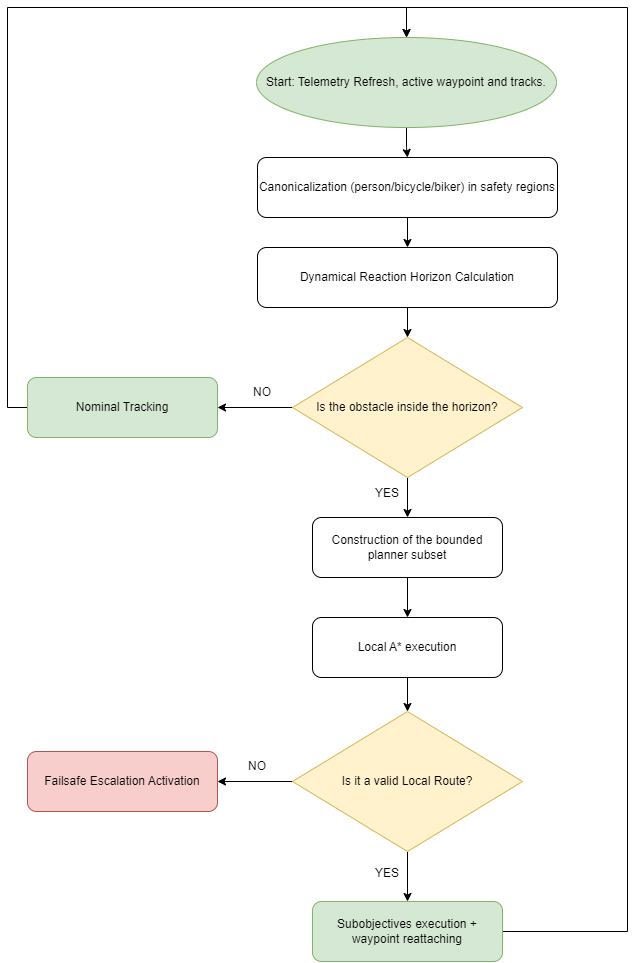
\includegraphics[width=0.8\columnwidth]{Main/images/System_Workflow.png}
    \caption{System \deleted{Workflow}\added{workflow} of the \deleted{Proposed}\added{proposed} PORCE \deleted{Control Loop}\added{control loop}}
    \label{solution}
\end{figure}
\reviewnote{Esta figura todav\'ia la tenemos que simplificar: menos texto dentro de las cajas y letra bastante m\'as grande. El flujo deber\'ia quedarse en algo tipo telemetr\'ia/percepci\'on $\\rightarrow$ trigger $\\rightarrow$ A* local $\\rightarrow$ evasi\'on/reattachment $\\rightarrow$ failsafe si falla (R4-D4, R2-6).}

However, as introduced in Section~1, the operational focus shifts during execution. At this stage, residual conflicts can arise from uncertain or locally perceived conditions that cannot be fully represented during pre-flight planning. \deleted{In these circumstances, simplified assumptions are often adopted, along with a neglect of regulatory compliance considerations. The proposed}\added{PORCE provides a} local reactive \deleted{navigation model enables realistic adaptation in real-time to the environment.}\added{layer that modifies the horizontal reference trajectory when newly perceived protected entities conflict with the nominal mission corridor. This behavior is regulation-aware in motivation, but it is not a substitute for the complete operational risk assessment.}


The logic at the controller level that constitutes the scientific core of the proposed method is summarized in Figure~\ref{solution}. At each iteration, the method receives the active waypoint, fresh perception outputs, and current telemetry. Civilian-like detections are converted into protected local regions. If the nearest obstacle enters the dynamic reaction horizon, the method activates a  bounded A* local bypass; otherwise, it preserves the nominal mission following. 


\subsection{Problem Formulation}
At each control iteration, PORCE knows the current vehicle state, the active mission waypoint, and the most recent obstacle list. The method is only concerned with the local subproblem: move from the current position to the current waypoint while avoiding the obstacle subset that lies inside a bounded planning neighborhood.

%ESTÁ MUY BIEN ESTE PARRAFO PERO LE DARÍA ALGO MÁS DE VALOR CON EL REFRENDADO EN LA NORMATIVA O BASADO EN LA EXPERIENCIA PRÁCTICA DE LO QUE ESTAMOS HABLANDO: QUE NO QUEREMOS PERDER EL OBJETIVO FUNDAMENTAL DE LA MISIÓN QUE ES LA CAPTURA DE DATOS. POR OTRO LADO TAMBIÉN QUEREMOS "QUE EL METODO NO AMPLIE EL CONSUMO" Y TAL COMO FUNDAMENTA EL PAPER AQUÍ MENCIONADO HACER CAMBIOS DE ALTURA PUEDE LLEGAR A CONSUMIR MÁS POTENCIA QUE HACER CAMBIOS DE DIRECCIÓN. "El estudio empírico de referencia, titulado An Empirical Study on Generic Multicopter Energy Consumption Profiles (por Stolaroff et al.), analiza detalladamente cómo varían los perfiles de consumo según el ángulo de inclinación de la trayectoria. En este trabajo se demuestra empíricamente que los picos más altos de consumo de energía eléctrica ocurren en las maniobras de cambio de altura (ascenso vertical), superando notablemente al consumo en traslación horizontal." REFERENCIA: https://ieeexplore.ieee.org/abstract/document/7934762/ \cite{dietrich2017empirical}

\added{Planning is formulated in the horizontal plane at the current mission altitude. The protected entities considered in the present implementation are treated as ground-based obstacles, and the avoidance maneuver does not optimize altitude. Consequently, the local PORCE planner preserves the mission altitude and modifies only the horizontal path. This scope choice reduces the online search space and keeps the local planner deterministic and bounded, but it also means that obstacles intersecting the flight level or scenarios requiring vertical avoidance are outside the demonstrated operational envelope.}


Let the vehicle position be \(p_t \in \mathbb{R}^2\), the current waypoint be \(w_t \in \mathbb{R}^2\), and the perceived obstacles at time \(t\) be \(\mathcal{O}_t = \{o_1,\dots,o_k\}\). Each obstacle is inflated by a hard safety radius \(R_s\), generating a non-flyable region
\begin{equation}
    \mathcal{Z}_{\mathrm{safe}}(o_i) = \{q \in \mathbb{R}^2 : \lVert q - p_{o_i} \rVert_2 \le R_s\}.
\end{equation}

The local free space is therefore
\begin{equation}
    \mathcal{F}_t = \mathbb{R}^2 \setminus \bigcup_{i=1}^{k} \mathcal{Z}_{\mathrm{safe}}(o_i).
\end{equation}

In the current implementation, $R_s = 12~m$, which turns safety into a hard geometric constraint instead of a soft penalty.

The value is a conservative operational heuristic, not a quantity derived from the SORA critical-area model\deleted{: it}\added{. It} is intended to \deleted{absorb the monocular geopositioning error of the perception front-end, the tracking and execution tolerance of the controller, and a regulatory}\added{cover, in a single design} margin, \deleted{all at once.}\added{perception/geopositioning uncertainty and tracking/execution tolerance; these contributions have not yet been separately quantified in the supplied evidence. We therefore do not interpret the residual margin as a formal regulatory buffer.} The implementation already supports class-dependent radii; the static campaign reported here uses \deleted{the value of}\added{a} 12~m \added{radius for the }livestock\added{ class}.

\reviewnote{Aqu\'i nos falta cerrar de verdad por qu\'e son 12~m. Tenemos que juntar el error de geoposicionamiento contra ground truth, error de seguimiento, latencia percepci\'on--decisi\'on, FOV/rango real de la c\'amara y capacidad de frenado/maniobra. Adem\'as, el revisor pide sensibilidad: variar $R_s$, $D_{base}$, $k_v$ y/o velocidad y ver c\'omo cambian clearance, ruta y tiempo. Si esto no est\'a ya en los logs, tenemos que hacer nuevas ejecuciones (R3-2, R4-D10, R4-E5).}



Other solutions presented in the earlier analysis of the state of the art present more general continuous cost-shaping ideas, including barrier-style formulations, as possible future directions. The system analyzed here \deleted{is more focus on other aspects}\added{focuses instead on a different design point}: a deterministic bounded grid planner with hard obstacle inflation and explicit failsafe escalation, not a Control Barrier Function controller.

\subsection{Dynamic Triggering Logic}

The method is not permanently active. The controller computes a dynamic reaction horizon
\begin{equation}
    D_{\mathrm{react}}(t) =
    \mathrm{clip}\!\left(D_{\mathrm{base}} + k_v \lVert v_t \rVert_2,\,
    D_{\min},\, D_{\max}\right),
\end{equation}
where $\lVert v_t \rVert_2$ is the horizontal ground-speed norm reported by autopilot telemetry, $D_{\mathrm{base}}=45~m$, $k_v=2.0~s$, $D_{\min}=45~m$, and $D_{\max}=80~m$.

The horizon \deleted{can be read}\added{is designed} as a \deleted{stopping-and-reaction}\added{conservative reaction} budget: \deleted{the}\added{a fixed} base distance \deleted{covers the detection-to-decision latency of the 10~Hz control loop plus a conservative braking margin at the 8~m/s cruise speed, and the speed gain enlarges it}\added{is enlarged} linearly with \deleted{the actual}\added{measured} ground speed\deleted{.}\added{ and clipped to the configured operating range. The present manuscript does not yet claim that the constants are derived from measured perception latency or braking dynamics.} The lower clip bound coincides with $D_{\mathrm{base}}$ and \deleted{acts as a guard against negative}\added{enforces a minimum reaction horizon even when the measured ground-speed norm is small} or noisy\deleted{ speed estimates, so the horizon never shrinks below the base distance.}\added{; because $\lVert v_t\rVert_2$ is a norm, it is non-negative by definition.}


If the nearest perceived obstacle satisfies
\begin{equation}
    d_{\mathrm{nearest}}(t) \le D_{\mathrm{react}}(t),
\end{equation}
and the minimum replan interval has elapsed, PORCE requests a new local route from the replanning module. Otherwise, the vehicle continues nominal waypoint following.

The trigger is deliberately direction-independent: any obstacle inside the horizon, not only obstacles on the flight path, can request a replan, and the bounded planner itself decides whether a detour is geometrically necessary. Once a valid evasion route exists, the evasion state is latched: it persists until the local route is exhausted, so the avoidance behavior can continue after the obstacle has left the horizon. While the evasion state is active, replanning is allowed at most once per minimum replan interval.

\subsection{Bounded Local A* Planner}

The method uses a local occupancy grid centered on the vehicle. The \deleted{validated }configuration \deleted{uses}\added{used in the reported experiments contains} \(81 \times 81\) cells with $\delta=6~m$ resolution (a 40-cell radius around the vehicle)\deleted{, resulting in a bounded search window that is compatible with online execution inside the control loop.}\added{. This bounds the search space, but the present manuscript does not yet provide a sensitivity analysis or measured planner runtime demonstrating that this grid is an optimal or validated configuration.}



\added{Only obstacles within 55~m of the vehicle are handed to the local planner, with the planner input capped at 16 tracks; the obstacle that triggers a replan is force-included in the subset even when it lies beyond that gate. Two boundary cases are treated explicitly. If the active mission waypoint lies outside the 40-cell local window, the goal is projected to the grid boundary along the waypoint direction. If the projected goal lies inside an inflated obstacle region, the nearest free cell within the configured boundary-search neighborhood is substituted. Conversely, if the start cell is occupied because the vehicle has entered an inflated region before replanning is triggered, the start cell is released to permit an escape route. With $\delta=6~m$, the cell-intersection test can conservatively add up to half a cell diagonal ($\delta\sqrt{2}/2\approx4.2~m$) to the nominal obstacle inflation; therefore the effective discretized exclusion margin may exceed the configured 12~m radius.}



Each cell \(c_{ij}\) is labeled as free or occupied according to the inflated obstacle set:
\begin{equation}
    S(c_{ij}) =
    \begin{cases}
        1, & \text{if } c_{ij} \cap \left(\mathbb{R}^2 \setminus \mathcal{F}_t\right) \neq \varnothing,\\
        0, & \text{otherwise.}
    \end{cases}
\end{equation}

The local route is computed with A* \cite{hart1968formal} using Euclidean heuristic,
\begin{equation}
    f(n) = g(n) + h(n),
\end{equation}
where \(g(n)\) is the cost of the accumulated path and \(h(n)\) is the Euclidean distance to the local goal. Eight-connectivity is enabled, so the method can combine cardinal (cost $\delta$) and diagonal moves (cost $\delta\sqrt{2}$) while remaining on the grid.

The target of the method is always the \emph{current mission waypoint}. This detail is important: the local planner is not allowed to redefine the global mission, only to create a temporary bypass that lets the UAV return to the original corridor as soon as the conflict disappears. \added{Using the already active mission waypoint as the local goal also gives PORCE a simple reattachment rule: the local planner does not need to select a new terminal waypoint or solve a second global planning problem after each conflict.}

\subsection{Nominal Navigation, Temporary Inhibition, and Route Reattachment}

The method should be understood as a \emph{temporary inhibition} of nominal navigation rather than as a new mission planner. 

Inside the control loop, the detection function is activated, so the system will continuously check the state of the obstacles with the detection function ($get\_detection$). The system responsible for providing the input to this function is an RGB camera board in the UAS. \deleted{The methodology used}\added{The} detection \deleted{of non regulatory compliant items or}\added{and tracking of protected entities and} physical obstacles \deleted{is based on the tracking}\added{follow the approach} proposed \deleted{on}\added{in} \cite{alaez2023real}.

\deleted{This detection function is the key element to select the path inside the control loop. If}\added{The current obstacle state determines whether PORCE keeps the nominal waypoint-following flow or activates local replanning. When} no conflict is \deleted{detected, the system executes the}\added{present,} nominal navigation \deleted{flow following the previously planned trajectory. The nominal navigation works}\added{proceeds} as follows: 
\begin{itemize}
    \item If $current\_idx$ is less than the length of the proposed \deleted{Flight Plan}\added{flight plan}, the system continues on the planned flight path. At each iteration, it checks whether the distance to the current target waypoint is below a threshold tolerance; if so, the target is updated to the next waypoint for the subsequent iteration. 
    \item If not, the last waypoint of the \deleted{Flight Plan}\added{flight plan} is reached, so the \deleted{Mission}\added{mission} terminates through the landing logic.
\end{itemize}

Conversely, when the nearest obstacle crosses the dynamic reaction horizon, this nominal flow is suspended, and an evasion path becomes the active short-horizon reference path. During that interval, the aircraft no longer tries to cut through the original corridor; instead, it follows the local sub-goals returned by the bounded A* planner. As soon as that local path is exhausted, nominal waypoint following resumes automatically toward the same \deleted{Mission}\added{mission} waypoint that was active before the conflict.

This behavior is operationally \deleted{important for powerline}\added{useful for power-line} inspection\deleted{. The objective of the method is not merely to avoid collisions, but to resolve}\added{ because the} local \deleted{conflicts in real time}\added{planner resolves a conflict without redefining the global mission}. Once \deleted{safe conditions are restored, the system}\added{the evasion route is exhausted, control} returns to the \deleted{globally planned route as quickly as possible. In this way, operational}\added{active mission waypoint. The current simulation evidence shows a small path-length increase in the complete evasion runs, but it does not establish a general guarantee of} safety \deleted{is maintained without compromising the}\added{or zero} efficiency \deleted{objective defined during the initial global planning stage, whether optimized data acquisition, Mission progression, or any}\added{loss across} other \deleted{Mission-specific metric established a priori.}\added{scenarios.}

\subsection{Failsafe Escalation}

If no valid local route is found, PORCE does not continue nominal flight blindly. The system integration includes an explicit escalation chain with hold, lateral replan, and terminal \texttt{LAND}/\texttt{RTL} actions. This failsafe design is part of the method even when it is not triggered in a particular experiment because it bounds the controller behavior under planner failure. \added{In the reported configuration, a planner failure with the nearest obstacle inside 22~m first commands a 2.5~s hold and retries planning. Repeated failures within a 12~s window escalate the response: the first failures each command a fresh 2.5~s hold at the vehicle's current position, from the third failure the escalation stage is \texttt{HOLD}, at the fifth failure a lateral replan with a 22~m offset is attempted, and at the sixth failure the terminal action is \texttt{LAND}, with \texttt{RTL} available as a configurable alternative. A 20~s cooldown bounds re-entry into the escalation chain.} \reviewnote{Esta parte est\'a implementada, pero en la campa\~na que tenemos no se activ\'o la cadena de failsafe. Si queremos decir que el failsafe est\'a validado, nos faltan ensayos forzando fallos de planner; si no, lo dejamos como comportamiento implementado pero no validado.}

% NO SE SI LA PARTE AÑADIDA AQUÍ TIENE SENTIDO, PUESTO QUE AL NO TENER OBSTÁCULOS EN MOVIMIENTO, EL SISTEMA VA A ACABAR EJECUTANDO UN FAILSADE SIEMPRE, Y QUIZÁS NO TIENE SENTIDO DAR MÁS EXPLICACIÓN DE QUE EJECUTA EL FAILSAFE SI NO ECUENTRA RUTA POSIBLE Y LISTO. POR OTRO LADO, DE DÓNDE SALE EL OFFSET DE 22 m? 


\subsection{Algorithmic Summary}
Listing\deleted{ }\added{~}\ref{lst:control} summarizes the \deleted{complete}\added{PORCE} control \deleted{loop of the proposed method, integrating the nominal navigation, dynamic triggering, bounded replanning}\added{logic as implementation-independent pseudocode, separating inputs, trigger evaluation, local planning, route execution}, and failsafe \deleted{escalation described in Sections 2.1--2.5.}\added{behavior.}

\begin{lstlisting}[caption=\added{Implementation-independent pseudocode of the PORCE control loop}, label=lst:control, basicstyle=\ttfamily\footnotesize\color{green!50!black}, keywordstyle=\color{green!50!black}, commentstyle=\color{green!50!black}, stringstyle=\color{green!50!black}]
INPUT: mission waypoints, vehicle state, georeferenced obstacle tracks
PARAMETERS: safety radii, reaction-horizon constants, grid limits,
            waypoint tolerance, minimum replan interval
OUTPUT: nominal waypoint reference, evasion sub-point, or failsafe action

initialize mission index and controller state
while mission is active:
    refresh telemetry and obstacle tracks
    if telemetry is stale:
        skip this control iteration

    if a failsafe action is active:
        execute the active failsafe action
        continue

    goal <- current mission waypoint
    D_react <- speed_adaptive_reaction_horizon(groundspeed)
    obstacle <- nearest protected track

    if obstacle exists and distance(obstacle) <= D_react
       and replanning is allowed:
        subset <- bounded_planner_obstacle_subset()
        route <- bounded_A_star(current_position, goal, subset)
        if route is valid:
            activate_or_update_evasion(route)
        else:
            escalate_failsafe_state()

    if an evasion route is active:
        command next evasion sub-point
    else:
        command current mission waypoint
        if mission waypoint is reached:
            advance mission index

terminate through the nominal mission landing/terminal logic
\end{lstlisting}

\reviewnote{Hemos cambiado el listing a pseudoc\'odigo de algoritmo y no a c\'odigo Python. Si necesitamos un formato todav\'ia m\'as acad\'emico tipo Algorithm/Algorithmic, podemos pasarlo luego a ese entorno, pero la l\'ogica ya est\'a separada de detalles de implementaci\'on (R4-D5).}

\section{Experimental Setup}
\subsection{Method Integration in Simulation Workflow}
\label{sec:Sim_workflow}
The proposed method is evaluated inside \deleted{a validated \texttt{SIMULATION}}\added{the simulation} workflow\deleted{.}\added{ described below.}

The runtime architecture is \deleted{specified in the figure }\added{shown in Figure~}\ref{fig:simulation_architecture}. The \deleted{Mission}\added{mission} is read from a QGroundControl waypoint file, vehicle state is received from the software-in-the-loop (SITL) through MAVLink, obstacles are produced by the vision module, and the PORCE system coordinates the nominal waypoint following, replanning activation, and visualization outputs. All components run as separate processes on the host machine: the ArduPilot SITL instance, the PORCE control process (labeled BRAIN, the historical name of the controller module, in Figure \ref{fig:simulation_architecture} and in the log prefixes), the vision front-end, and the visualization endpoint, connected through MAVLink over TCP and local HTTP interfaces.

\begin{figure}[h!]
\centering
\captionsetup{justification=centering}
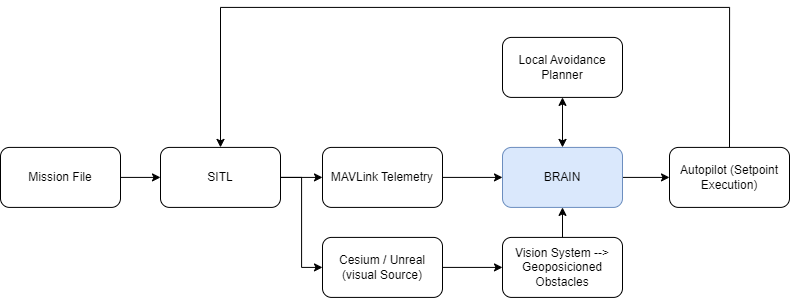
\includegraphics[width=0.7\columnwidth]{Main/images/Pipeline_A.png}
\caption{\deleted{Simulation Environment Diagram}\added{Runtime architecture of the simulation workflow}}
\label{fig:simulation_architecture}
\end{figure}

\deleted{The Simulation Environment roles}\added{The main simulation-workflow components} are the following:

\begin{itemize}
    \item \textbf{Mission input:} This is the file that contains the nominal inspection route.
    \item \textbf{SITL:} Software-in-the-loop simulation.
    \item \textbf{MAVLink telemetry}: vehicle state stream relayed from the SITL autopilot to PORCE and to the vision front-end.
    \item \textbf{Cesium / Unreal Engine simulator}: \deleted{It is the}\added{This component provides the georeferenced} visual \deleted{Source of the environment.}\added{environment used by the simulated perception chain.}\reviewnote{Aqu\'i nos faltan el nombre y la versi\'on exactos de Unreal Engine y Cesium for Unreal. No los damos por hechos: tenemos que sacarlos del proyecto o del equipo donde se hicieron los ensayos (R4-A2).} 
    \item \textbf{PORCE:} executes the control loop, manages waypoints, handles failsafe logic, and calls the replanning module whenever local replanning is necessary.
    \item \textbf{Perception:} runs a YOLO-based detector and projects detections in geographic coordinates using onboard state and the monocular geometry \cite{alaez2023real}. The detector uses the repository weights trained on the Unreal Engine simulator inspection scene, a detection confidence threshold of 0.10, a publish threshold of 0.35, and a minimum of three observations before a track is published. It is part of the PORCE control loop.
    \reviewnote{Aqu\'i nos faltan n\'umeros de percepci\'on. Los thresholds dicen c\'omo est\'a configurado YOLO, pero no dicen si detecta bien. Tenemos que meter precision/recall/mAP o TP--FP--FN y el error horizontal del geoposicionamiento contra ground truth. Para robustez de verdad tambi\'en nos faltan pruebas metiendo error/ruido de forma controlada (R4-E5, R3-4).}
 
    \item \textbf{Local Avoidance Planner:} This function implements the bounded A* local planner used to generate short-range evasion paths. It is part of the PORCE control loop. 
    \item \textbf{Visualization:} the visualization endpoint \deleted{expose}\added{exposes} the evolution of the \deleted{Mission}\added{mission} for analysis and debugging.
    \item \textbf{Autopilot}: \deleted{It }runs inside SITL and executes the \added{position }setpoints \deleted{position.}\added{issued by the guidance layer.} 
\end{itemize}

\added{Table~\ref{tab:runtime_configuration} collects the main runtime parameters used by the reported static-obstacle configuration.}

\begin{table}[h!]
\centering
\caption{\added{Main PORCE runtime parameters used in the reported static-obstacle configuration.}}
\label{tab:runtime_configuration}
\small
\begin{tabular}{ll}
\toprule
\textbf{Parameter} & \textbf{Value}\\
\midrule
\added{Control-loop period} & \added{0.10~s (10~Hz)}\\
\added{Cruise speed} & \added{8~m/s}\\
\added{Local grid} & \added{$81\times81$ cells; 6~m/cell}\\
\added{Livestock safety radius} & \added{12~m}\\
\added{Reaction horizon} & \added{45--80~m; $k_v=2.0$~s}\\
\added{Minimum replan interval} & \added{1.0~s}\\
\added{Planner obstacle subset} & \added{55~m + trigger obstacle force-included; maximum 16 tracks}\\
\added{Route-point tolerance} & \added{3~m}\\
\added{Mission-waypoint tolerance} & \added{5.5~m}\\
\added{Track time-to-live} & \added{30~s static / 3~s dynamic}\\
\added{Failsafe threshold} & \added{22~m}\\
\bottomrule
\end{tabular}
\end{table}
\reviewnote{Los 10~Hz de la tabla son el periodo configurado del lazo, no una medida de tiempo de c\'omputo. Nos falta medir cu\'anto tarda realmente cada iteraci\'on y cada replan en el hardware embarcado, adem\'as de CPU/GPU/memoria, antes de defender rendimiento real-time cuantitativo (R3-6).}

\subsection{Method Integration within \deleted{a}\added{an} Experimental UAS Architecture}
\label{sec:uas_architecture_real}

The proposed method is further \deleted{evaluated}\added{exercised} in a controlled real-world environment following the \deleted{simulation-based validation}\added{simulation campaign}. For this purpose, it is integrated into the onboard UAS architecture shown in \deleted{the }Figure\deleted{ }\added{~}\ref{fig:real_world_architecture}. The architecture \deleted{is designed to manage all}\added{manages} the information \deleted{flow between}\added{exchanged among} the navigation, perception, guidance, and control modules required for \deleted{Mission}\added{mission} execution. \deleted{Within this framework, the proposed guidance algorithm is incorporated}\added{PORCE runs} as part of the \added{onboard }decision-making \deleted{process onboard and interacts}\added{chain and exchanges vehicle-state information and trajectory references} with the remaining components\deleted{ to generate and update trajectory references during flight.}\added{.}

\reviewnote{Aqu\'i nos faltan los datos de hardware y versiones: modelo de UAS, autopiloto, ordenador embarcado (CPU/GPU/RAM), c\'amara, resoluci\'on/FPS/FOV, versi\'on de ArduPilot y versi\'on exacta de Unreal/Cesium. Tambi\'en tenemos que poner cu\'antos vuelos/repeticiones hicimos. Sin esto no podemos cerrar bien el comentario de tiempo real y reproducibilidad (R3-6, R4-E1, R4-A2).}

%TODAS LAS COSAS SE PUEDEN SACAR EN TEÓRICO AUNQUE REALMENTE NO LAS HAYAMOS UTILIZADO. EL UNREAL CREO QUE NO HACE FALTA PARA ESTO. 


The main elements of the UAS architecture and their roles are described below: 
\begin{itemize}
    \item \textbf{Mission input:} File \deleted{that contains}\added{containing} the nominal inspection route used as the \added{mission }reference\deleted{ Mission} for the UAS.
    \item \textbf{Visual camera:} \deleted{Provides}\added{provides} the image stream used to monitor the surrounding environment and supplies the visual data required by the YOLO-based detection module.
    \item \textbf{GNSS and compass unit:} \deleted{Provides}\added{provides} the global positioning and heading measurements required by the onboard navigation systems. These measurements contribute to the vehicle state estimate used by the proposed guidance method to determine the UAS state with respect to the \deleted{Mission}\added{mission} reference frame. 
    \item \textbf{Onboard computer:} \deleted{Hosts}\added{hosts} the main onboard software components of the PORCE solution and the YOLO-based detector. The onboard computer communicates directly with the autopilot through MAVLink to exchange vehicle-state information and trajectory references. 
    \item \textbf{YOLO-based detector:} \deleted{Runs}\added{runs} on the onboard computer. This module projects image detections into geographic coordinates using onboard state and the monocular geometry \cite{alaez2023real}. The detector uses network weights trained on the previous simulation workflow, with a detection confidence threshold of 0.10, a publish threshold of 0.35, and a minimum of three observations before a track is published. The resulting detections are subsequently incorporated into the PORCE guidance loop.
    \item \textbf{PORCE:} \deleted{Runs}\added{runs} on the onboard computer\deleted{. PORCE}\added{,} executes \deleted{onboard}\added{the} guidance and \deleted{Mission-management}\added{mission-management} loop, manages the mission waypoints, handles the associated failsafe logic, and invokes the replanning module whenever a local trajectory modification is required. 
    \item \textbf{MAVLink telemetry:} \deleted{Communication}\added{communication} stream used to relay \deleted{vehicle state}\added{vehicle-state} and navigation information from the ArduPilot autopilot to the onboard computer.
    \item \textbf{ArduPilot autopilot:} \deleted{Runs}\added{runs} the ArduPilot flight-control software of the UAS and is responsible for executing the position setpoints provided by the onboard guidance and \deleted{Mission-management}\added{mission-management} architecture.  
\end{itemize}

\begin{figure}[h!]
\centering
\captionsetup{justification=centering}
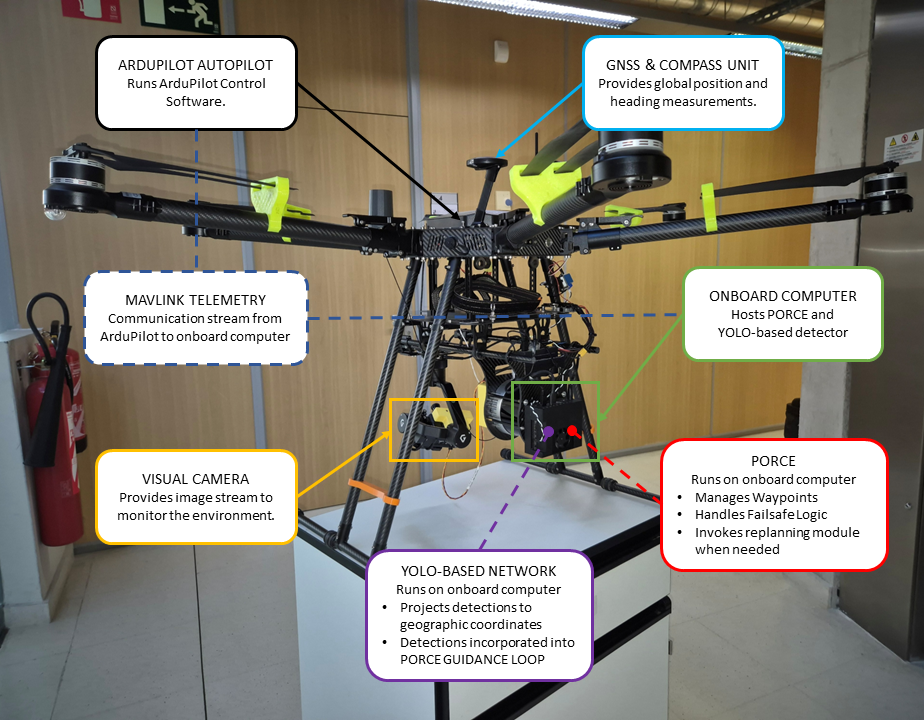
\includegraphics[width=0.7\columnwidth]{Main/images/real_world_workflow.png}
\caption{\added{Onboard }UAS architecture \deleted{for Real-world environment}\added{used for the real-world field campaign}}
\label{fig:real_world_architecture}
\end{figure}


\section{\deleted{Results}\added{Evaluation}}

This section \deleted{presents the results obtained during the validation of the proposed solution. It is divided into two main validation}\added{reports two evaluation} campaigns: the \added{logged static-obstacle }simulation campaign\deleted{, where the solution is tested inside the validated simulation workflow} described in \added{Section~}\ref{sec:Sim_workflow}\deleted{; and a static-obstacle}\added{ and the controlled field} campaign \deleted{in the field, where the solution is tested on a real UAS in a controlled scenario, as}\added{performed with the physical UAS architecture} described in \added{Section~}\ref{sec:uas_architecture_real}.

\subsection{\added{Controlled Planner Behaviour Analysis}}
\reviewnote{Aquí se incluye cómo responde el algoritmo frente a configuraciones controladas de obstáculos. Es decir, las diferentes casuísticas en un caso congelado del FOV de la cámara para ir introduciendo obstáculos y ver cómo se comporta de manera puramente teórica y en un entorno controlado dónde poder ir controlando el número de obstáucluos y representar distintas figuras con 1, vatrios obstáculos, distintas distribuciones, rutas alternativas generadas, casos que fuerzan una mayor desviación, y algún caso sin solución que genere un FAILSAFE. Objetivo de la sección: Explicar como se comporta gráficamente}

\section{\added{Monte Carlo Analysis}}

\reviewnote{aquí se incluye cómo se comporta estadísticamente el planificador y cómo degrada su rendimiento al aumentar la complejidad. Respondiendo a la pregunta científica de: How does the planner behave as the complexity of the local environment increases? Se presenta una tabla del tipo: " Across a 1000 randomized scenarios, increasing obstacle density reduced the feasible solution rate from X\% to Y\% and inctreased median replanning time from A ms to B ms. Ovjetivo de la sección: Cuantificar y generalizar el comportamiento de la solución}
\reviewnote{En ambas secciones propuestas la idea por detrás es que se trata de casos generados artificialmente en los que los obstáculos se colocan directamente para la representación y no hay una detección real con el sistema YOLO. Se trata de una representación de un caso "estático", con lo que eso conlleva a la hora de limitaciones en los resultados del estudio, porque se limita la "franja de escape" al escenario analizado que simula el detection range de la camara 150 m. }

\subsection{Simulation Campaign}
\reviewnote{En esta sección lo que se responde es: Can the complete system execute the proposed approach under representative inspection conditions?}

\added{The archived static-obstacle simulation campaign comprises twenty runs against the cattle scenario. Eight runs satisfy the objective criteria used for quantitative analysis: four runs in which the perception front-end published an obstacle and an evasion was triggered, and four runs over the same corridor with no published obstacle, used as the dormancy baseline. Runs with telemetry-integrity problems or incomplete traversal of the inspection corridor are not used for the principal mission-level comparison. The quantitative metrics extracted from the archived telemetry and decision logs include mission duration, flown path length, time spent in evasion, minimum logged distance to the nearest perceived obstacle, number of replan requests, and first-trigger distance.}
\reviewnote{Aqu\'i todav\'ia no llamamos a esto ``100\% success rate''. Sabemos que en las cuatro ejecuciones analizadas con obst\'aculo publicado se activ\'o la evasi\'on, pero dos son recorridos parciales y no hemos definido un criterio formal de \'exito/fallo para los veinte archivos. Si queremos publicar una tasa de \'exito, tenemos que fijar primero ese criterio y contar todos los casos de forma reproducible (R4-E3, R4-E6).}

\begin{table}[h!]
\centering
\caption{\added{Logged metrics retained from the original static-obstacle simulation campaign. Clearance is measured relative to the nearest perceived obstacle position.}}
\label{tab:v3_sim_metrics}
\small
\begin{tabular}{lrrrrr}
\toprule
\textbf{Run} & \textbf{Duration (s)} & \textbf{Path (m)} & \textbf{Evasion (s)} & \textbf{Min. perceived clearance (m)} & \textbf{Replans}\\
\midrule
\added{20260730\_232617} & \added{153.6} & \added{915.3$^{a}$} & \added{34.8} & \added{20.6} & \added{n.r.}\\
\added{20260731\_060411} & \added{205.8} & \added{1318.1$^{a}$} & \added{27.7} & \added{32.0} & \added{n.r.}\\
\added{20260731\_061815} & \added{576.5} & \added{1465.4} & \added{28.2} & \added{29.6} & \added{23}\\
\added{20260731\_062851} & \added{n.r.$^{b}$} & \added{1469.3} & \added{29.2} & \added{29.1} & \added{n.r.}\\
\added{No published obstacle ($n=4$)$^{c}$} & \added{195.2--625.9} & \added{1357.0--1459.7} & \added{0} & \added{--} & \added{0}\\
\bottomrule
\end{tabular}
\begin{flushleft}\footnotesize
\added{$^{a}$ Run terminated before the final waypoint (partial corridor). $^{b}$ Telemetry recorder remained active after landing; duration is not representative. $^{c}$ One recording stops after the final inspection waypoint before the return-and-landing leg; the other three are complete flights. n.r.: not recorded in the decision log.}
\end{flushleft}
\end{table}

\added{Across complete evasion runs, path length increased from the approximately 1459.6~m obstacle-free baseline to 1465.4--1469.3~m, corresponding to a detour cost of approximately 5.8--9.7~m (0.4--0.7\%), below 1\% of the mission path. Evasion segments lasted 27.7--34.8~s. The minimum logged distance to the nearest perceived obstacle was 20.6~m in the worst archived evasion run and 29.1--32.0~m in the complete encounters, always above the configured 12~m safety radius with respect to those perceived positions. In the audited run 20260731\_061815, 23 replan requests were logged over a 28.2~s evasion segment.}

\deleted{In this section, the results of the experiments performed}\added{The following analysis combines visual evidence from the simulated encounter} with the \deleted{environment defined in the simulation workflow are represented.}\added{quantitative metrics extracted from the archived telemetry and decision logs.}

\begin{figure}[h!]
\centering
\captionsetup{justification=centering}
\subfloat[\centering]{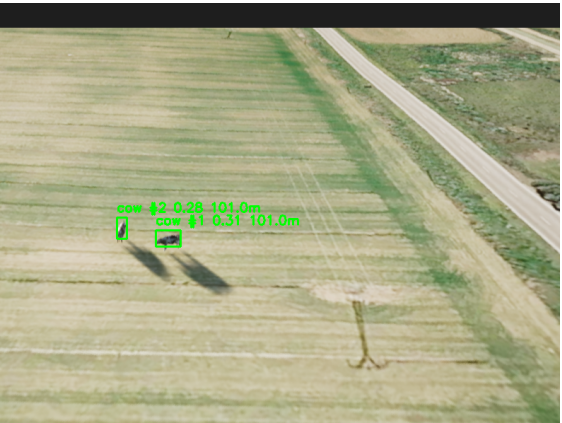
\includegraphics[width=0.32\textwidth]{Main/images/fig_static_perception_closeups_a.png}}
\hfill
\captionsetup{justification=centering}
\subfloat[\centering]{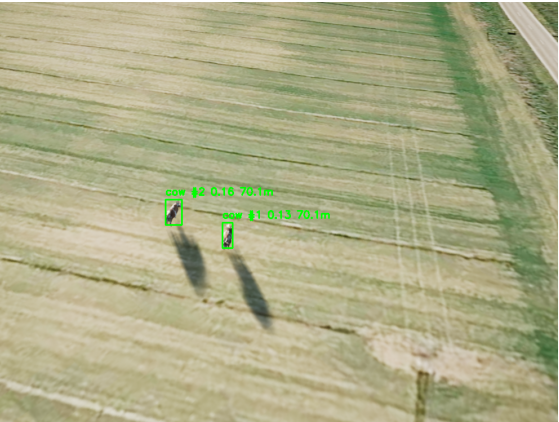
\includegraphics[width=0.32\textwidth]{Main/images/fig_static_perception_closeups_b.png}}
\hfill
\subfloat[\centering]{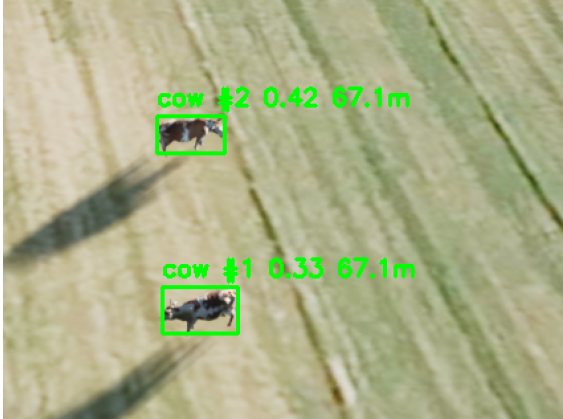
\includegraphics[width=0.32\textwidth]{Main/images/fig_static_perception_closeups_c.png}}\\
\caption{\added{Representative perception frames from the }Unreal Engine\deleted{ simulator Obstacles Detection Representation:}\added{/Cesium simulation environment:} \textbf{(a)} First obstacle detection. \textbf{(b)} Reaction-horizon entry. \textbf{(c)} Closest approach.\label{fig:Unreal_examples}}
\end{figure}

\deleted{As indicated in }\added{As described in Section~}\ref{sec:Sim_workflow}, the Unreal Engine\deleted{ simulation tool is used as}\added{/Cesium environment provides} the visual \deleted{source of the simulation environment. This tool makes it possible to recreate in this environment the real situation that is intended to be analyzed. In this case, for the recreation of the flight, static elements, such as cows and "uninvolved people" have been added, which represent elements that the UA must detect and avoid during the Mission. Figure \ref{fig:Unreal_examples} represents some images of the environment during the simulation, where it can be observed how this Unreal Engine simulation tool works and}\added{scene used by the perception front-end. The static campaign includes cattle positioned near the inspection corridor as protected obstacles. Figure~\ref{fig:Unreal_examples} shows representative perception frames from detection through closest approach and illustrates} how the \deleted{proposed solution is able to detect these obstacles and purpose an alternative route.}\added{perception output is linked to the replanning response.} 

\deleted{Once the operation of the solution has been represented visually, each and every one of the steps that take place during the validation of the method are described below. In this way, it can be checked whether the proposed solution is able to address the challenges for which it has been designed.}\added{The sequence below describes the same encounter from nominal waypoint following, through trigger activation and evasion, to route reattachment.} 

\deleted{In a first step, the Mission is downloaded into the}\added{The} simulated UAS\deleted{. The Mission comes from a preplanned waypoint file that contains a}\added{ loads a pre-planned mission containing} takeoff\deleted{ waypoint, a sequence of predefined}\added{,} inspection waypoints, and a landing command. \deleted{For the experiment, the UAS}\added{In the audited campaign, the aircraft} climbs from\added{ approximately} $500~m$ MSL to\deleted{ approximately} $523~m$ MSL, follows the inspection corridor, and \deleted{lands automatically once}\added{completes the terminal mission logic after} the final waypoint\deleted{ is reached. This initial planned behavior is represented in Figure \ref{fig:navigation_results} 1A, where it is notable that in}\added{. Figure~\ref{fig:navigation_results}a shows} the initial \deleted{stages the UAS is navigating without any perturbation, following the predefined waypoint path.}\added{nominal waypoint-following phase before local avoidance is activated.} 

\deleted{As explained before, while the UAS is in the air and, therefore, the proposed solution is running inside the embedded computer, the system is continuously analyzing the environment to detect if there is any}\added{While the mission is active, the perception front-end continuously updates the protected-obstacle tracks. Figure~\ref{fig:navigation_results}b shows an} obstacle \deleted{or non regulatory-compliant item that needs to be avoided. Figure \ref{fig:navigation_results} 1B represents the moment where the camera}\added{that} has already \added{been }detected \deleted{an obstacle (i.e. the obstacle is inside the Reaction Range), but the distance between the UAS and the obstacle still exceeds}\added{but remains outside} the reaction \deleted{distance. In this represented simulation at the}\added{horizon. At the nominal} cruise speed of $8~m/s$, \deleted{Equation (3)}\added{the configured trigger} gives \deleted{$D_{\mathrm{react}} = 45 + 2.0 \times 8 = 61~m$, so as the UAS is at 75 }\added{$D_{\mathrm{react}}=45+2.0\times8=61~m$; at approximately 75}~m from the obstacle, \deleted{the system is not yet computing an alternative evasion path and the obstacle remains only a potential hazard. The complete encounter, with the raw}\added{PORCE therefore remains in monitoring mode. Supplementary Video~S1 provides the corresponding} detection and tracking overlays\deleted{ produced by the vision front-end, is provided as Supplementary Video S1.}\added{.}

\begin{figure}[h!]
\centering
\captionsetup{justification=centering}

\includegraphics[width=\columnwidth]{Main/images/Imagenes_resultados_main.jpg}
\caption{\deleted{Navigation Results}\added{Simulation encounter: nominal flight, trigger, evasion, and route reattachment}}
\label{fig:navigation_results}
\end{figure}


\deleted{In contrast}\added{Figure~\ref{fig:navigation_results}c shows the later stage at which the obstacle enters the reaction horizon and triggers local replanning. The dashed circle represents the configured reaction boundary; the additional plotted margin is used only for visualization of position uncertainty. The controller then switches from nominal waypoint following} to the \deleted{previous paragraph and figure, where the obstacle had already been detected but remained outside the safety radius, Figure \ref{fig:navigation_results} 1C represents a later stage of the encounter. At this instant, the obstacle has entered the margins of the reaction distance (the dashed circle is the limit of the reaction radius, while the dot circle is an external limit taking into account the position error), triggering the trajectory replanning process. As a result, the system begins to compute an avoidance route designed to prevent a potential conflict and preserve the required separation margins.}\added{locally replanned bypass.}


\deleted{The visualization represented in }Figure\deleted{ }\added{~}\ref{fig:navigation_results}\deleted{ 1D therefore}\added{d} illustrates the transition from \deleted{a passive }monitoring \deleted{state, in which the obstacle is detected but no corrective action is required, to an active guidance state, in which the system evaluates the conflict and generates a feasible alternative path.}\added{to active local guidance after the trigger condition is met.}\deleted{In this case, the}\added{In the audited simulation run, the first} replan request is reported at \deleted{a nearest-obstacle distance of 60.7}\added{60.1}~m, consistent with the 61~m horizon predicted by Equation~(3)\deleted{.}\added{ at the 8~m/s cruise speed.} \reviewnote{Aqu\'i tenemos una contradicci\'on que debemos confirmar en el log: V2 puso 60.7~m una vez, pero la tabla/figura de clearance y el run auditado usan 60.1~m. Hemos mantenido 60.1~m porque es el valor respaldado de forma consistente en la evidencia que tenemos, pero antes de enviar tenemos que mirar el log una vez m\'as.} The route proposed by the UAS is highlighted in orange, allowing the reaction response trajectory to be clearly distinguished from the original trajectory.

\deleted{In Figure \ref{fig:navigation_results} 1E, it is appreciable how the UA is performing the evasion maneuver through the alternative}\added{Figure~\ref{fig:navigation_results}e shows the aircraft executing the locally} generated \deleted{path,}\added{bypass} while the static obstacle remains tracked\deleted{ and no conflict is reported.}\added{.} 


Figure\deleted{ }\added{~}\ref{fig:navigation_results}\deleted{ 1F}\added{f} shows the \deleted{complete resolution}\added{end} of the \added{local }conflict\deleted{, once the UAS has successfully rejoined its original path and can continue with the data acquisition Mission. At this stage, the avoidance maneuver}\added{: the evasion route} has been completed, \deleted{and the vehicle has returned to}\added{the aircraft has reattached to the} nominal \deleted{operation, resuming the planned inspection or monitoring task. This moment represents the final phase of the guidance response, where the temporary deviation introduced to maintain safe separation is no longer required and the Mission can proceed under normal conditions.}\added{mission corridor, and waypoint following resumes.}

\begin{figure}[h!]
\centering
\captionsetup{justification=centering}
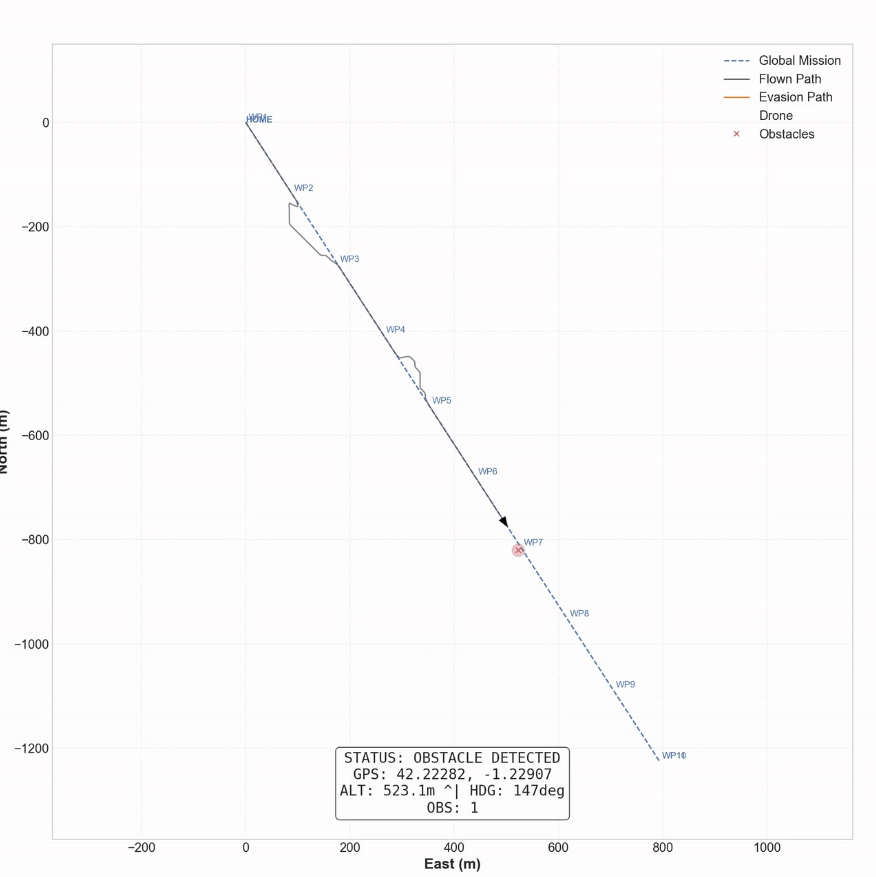
\includegraphics[width=0.7\columnwidth]{Main/images/transcurso_de_mision_(nuevo_obs_detectado).png}
\caption{\deleted{Middle Stages. Rejoining and new detections}\added{Route reattachment and continued obstacle monitoring after the first evasion}}
\label{fig:middle_stages}
\end{figure}

At this point, the incident is also recorded and reported by the system for subsequent analysis. Although this may result in partial data loss or gaps in the information collected from the asset during the maneuver, such limitations are considered acceptable within the operational framework. In safety-critical applications, preservation of the integrity of the UAS and maintaining a safe distance from obstacles must be the priority over uninterrupted data collection. Therefore, the figure not only illustrates the successful completion of the conflict-resolution but also highlights the underlying operational principle that Mission continuity is always subordinated to safety requirements.

Moreover, Figure \ref{fig:middle_stages} \deleted{also }shows that \deleted{the process does not remain as an isolated event. A new detection can be observed}\added{obstacle monitoring continues} after the UAS has returned to its nominal trajectory\deleted{, demonstrating that the system is not limited to a single conflict-resolution cycle. Instead,}\added{. The controller can therefore re-enter the detection--replanning--reattachment cycle when a subsequent protected region is encountered. This observation demonstrates repeated activation of the implemented state-transition logic in the reported scenario;} it is \deleted{capable of repeatedly transitioning between normal path-following, obstacle detection, trajectory replanning, and recovery to the original route as many times as required by the operational scenario. This behavior confirms the robustness and repeatability of the guidance strategy, showing that the UAS can respond consistently to successive conflicts without any inherent limitation in its ability to resume the Mission and reinitiate the avoidance process whenever necessary.}\added{not, by itself, a statistical demonstration of robustness under perception error, positioning error, multiple-obstacle density, or dynamic-target uncertainty.} \reviewnote{Aqu\'i no podemos decir todav\'ia que hemos demostrado ``robustness'' o ``repeatability'' en sentido estad\'istico. Nos faltan repeticiones y pruebas metiendo errores de detecci\'on/geoposicionamiento, y luego sacar tasa de \'exito y distribuci\'on de clearances/tiempos (R4-E7, R3-4).}

\begin{figure}[h!]
\centering
\captionsetup{justification=centering}
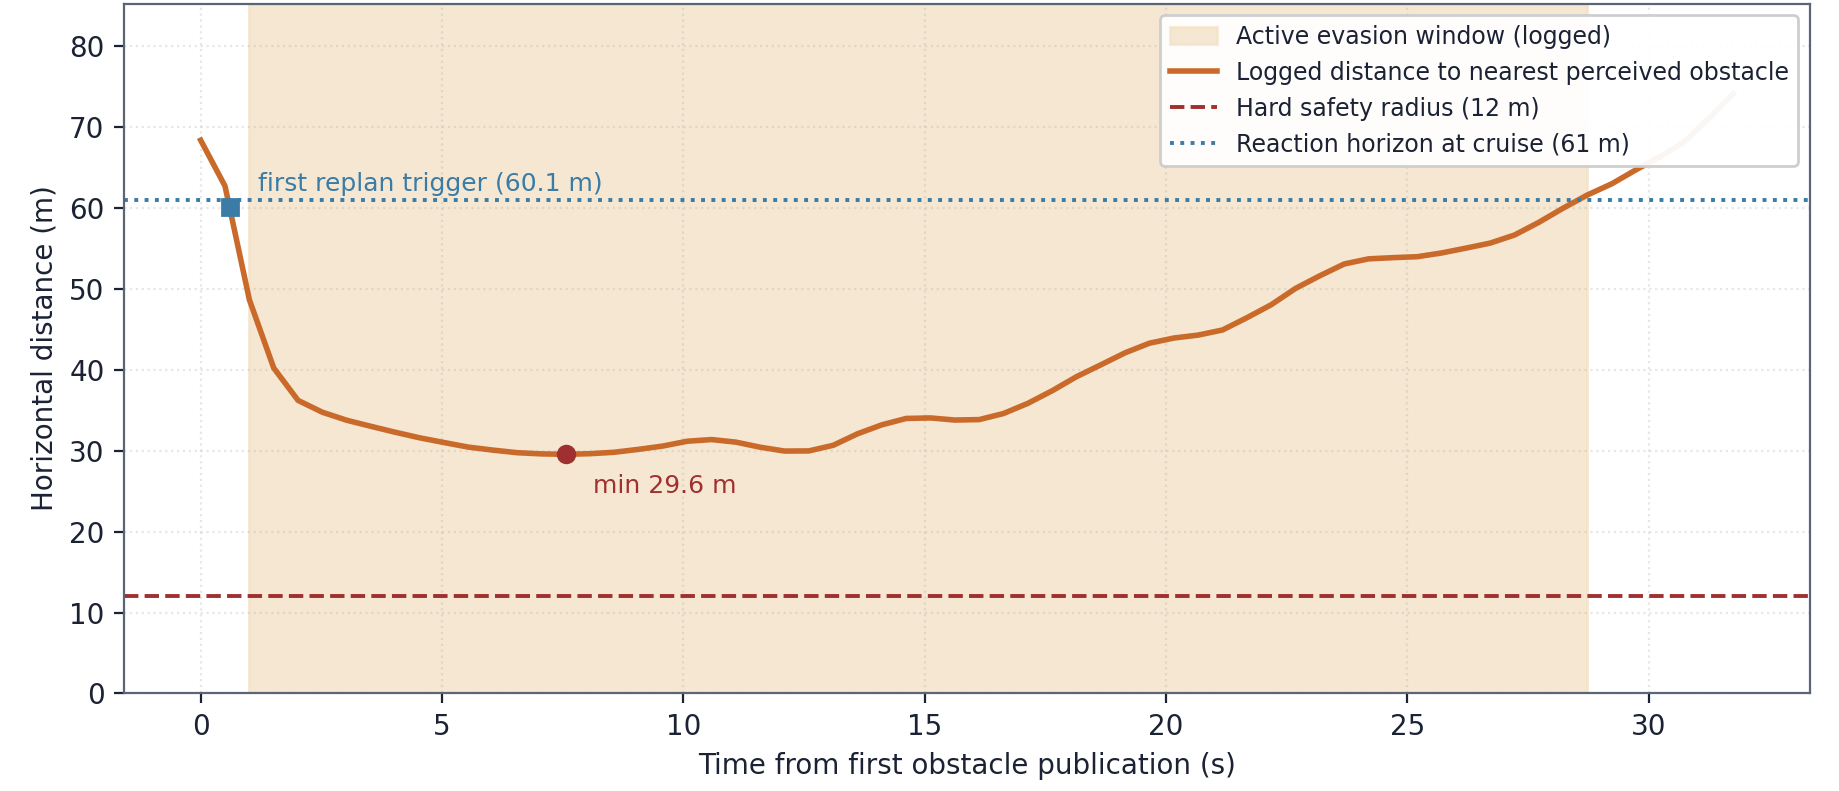
\includegraphics[width=\columnwidth]{Main/images/fig_static_clearance_timeseries_cut.png}
\caption{Logged clearance to the nearest perceived obstacle during the \deleted{different}\added{audited} simulated \deleted{runs}\added{encounter}}
\label{fig:clearance}
\end{figure}

Figure\deleted{ }\added{~}\ref{fig:clearance} plots the \added{logged horizontal }clearance\deleted{ logged} to the \deleted{closest}\added{nearest} perceived obstacle \deleted{over time for the different simulation runs. The series crosses the reaction horizon of 61 m  at the}\added{during the audited encounter. The} first replan \deleted{request (}\added{is recorded at }60.1\deleted{ ~m), stays far above the 12 ~m hard safety radius during the whole maneuver - within a}\added{~m, close to the configured 61~m reaction horizon, and the} minimum \deleted{29.6 ~m inside}\added{clearance during} the active evasion window \deleted{- and grows}\added{is 29.6~m, above the 12~m configured safety radius. The clearance increases} again as the vehicle \deleted{rejoins}\added{reattaches to} the corridor and the obstacle track expires.

\deleted{After that evaluation of these results derived from the different simulations performed, it can be concluded that the system works properly in a simulated workflow scenario.}\added{The logged simulation campaign therefore supports the specific behaviors evaluated here: dormancy outside the trigger condition, bounded evasion after activation, maintained clearance relative to perceived obstacle positions, and return to the nominal mission route.} 

\subsection{On the Field Campaign}
\reviewnote{Aquí la pregunta a resolver es: Does the behaviour observed in simulation transfer to an actual UAV platform?}

\deleted{In this section, the results of the experiments performed in the}\added{This subsection reports the controlled} field campaign \deleted{are presented.}\added{performed with the physical UAS.}

\reviewnote{Aqu\'i nos falta convertir la campa\~na real en una tabla como la de simulaci\'on: n\'umero exacto de vuelos, cu\'antos salieron bien/mal, clearance m\'inimo, tiempo de planning/replanning, desv\'io respecto a la ruta nominal, longitud, duraci\'on, tasa de completitud y consumo si lo registramos. Los vuelos existen y se quedan, pero sin esos n\'umeros la validaci\'on real sigue siendo demasiado cualitativa (R4-E1, R4-E3, R4-E6, R2-8, R1-5).}


The objective\deleted{ of these results} is to \deleted{validate in a real world scenario}\added{verify} that the PORCE \deleted{solution is working as demonstrated in the simulated workflow scenario.}\added{decision chain can be executed onboard in a real-world scenario and that the aircraft can perform the detection--evasion--reattachment sequence observed in simulation.} 

For the real-world scenario, the nominal mission is also uploaded to the autopilot. The Mission comes from a preplanned waypoint file that contains a takeoff waypoint, a sequence of predefined inspection waypoints, and a landing command. For the experiment, the UAS climbs from $287~m$ MSL to approximately $307~m$ MSL, follows the mission corridor (WP 2 to 4), and returns to the takeoff point to land once the final waypoint (WP 4) is reached. \added{The return/landing segment belongs to the mission/autopilot execution logic; PORCE does not plan or optimize a dedicated landing trajectory in the present implementation.}

\begin{figure}[h!]
    \centering
    \captionsetup{justification=centering}
    \subfloat[]{
        \includegraphics[width=0.3\linewidth]{Main/images/RW_trajectory_far_detection_g.JPG}
        \label{fig:img1}
    }
    \hfill
    \subfloat[]{
        \includegraphics[width=0.3\linewidth]{Main/images/RW_trajectory_starting_evasion_g.JPG}
        \label{fig:img2}
    }
    \hfill
    \subfloat[]{
        \includegraphics[width=0.3\linewidth]{Main/images/RW_trajectory_middle_evasion_g.JPG}
        \label{fig:img3}
    }

    \vspace{0.2cm}

    \subfloat[]{
        \includegraphics[width=0.3\linewidth]{Main/images/RW_trajectory_exit_evasion_g.JPG}
        \label{fig:img4}
    }
    \hfill
    \subfloat[]{
        \includegraphics[width=0.3\linewidth]{Main/images/RW_trajectory_middle_rejoin_g.JPG}
        \label{fig:img5}
    }
    \hfill
    \subfloat[]{
        \includegraphics[width=0.3\linewidth]{Main/images/RW_trajectory_rejoin_g.JPG}
        \label{fig:img6}
    }

    \caption{\deleted{Real World Scenario Different Stages:(a) Far Obstacle Detection, (b) Starting Evasion Stage, (c) Middle Evasion Stage, (d) Exiting Evasion Stage, (e) Starting Rejoin to Nominal Trajectory}\added{Real-world encounter stages: (a) far obstacle detection, (b) evasion activation, (c) and (d) evasion execution, (e) start of route reattachment}, and (f) \deleted{Nominal Trajectory Recovered}\added{nominal trajectory recovered.}}
    \label{fig:experimental_platform}
\end{figure}
\reviewnote{Aqu\'i ya hemos comprobado el PDF original: estas seis capturas del vuelo real no ense\~nan bounding boxes de YOLO equivalentes a las de simulaci\'on. Nos falta recuperar una captura o frame del stream real con las detecciones superpuestas; si ese material no existe, tendremos que reprocesar v\'ideo/frames guardados o repetir una adquisici\'on para cerrar R4-E2.}

Figure\deleted{ }\added{~}\ref{fig:experimental_platform} \deleted{represents the different moments that the camera has detected during the execution}\added{shows six stages} of the \deleted{Mission, when an obstacle appears. As described, in stage (a) the obstacle appears in the camera FOV, but the distance to}\added{physical-flight encounter. In panel (a),} the obstacle is \deleted{larger than the}\added{visible while it remains outside the configured} reaction horizon. \deleted{Stage (b) represents the starting of the}\added{Panel (b) corresponds to} evasion \deleted{stage, when the distance to the obstacle is less than}\added{activation after} the reaction \deleted{horizon distance. As expected, the system begins to compute the avoidance route intended to prevent a potential conflict and preserve the required separation margins. Stages}\added{condition is reached. Panels} (c) and (d) \deleted{are different evasion stages, once the evasion maneuver is already calculated and performed, maintaining the minimum safety distance and allowing to continue the Mission without violating the regulatory limitations. Stages}\added{show intermediate execution of the locally replanned path, and panels} (e) and (f) \deleted{represent the rejoining}\added{show route reattachment} and recovery of \deleted{the }nominal \deleted{trajectory, once the obstacle is cleared.}\added{mission following. These images document the maneuver sequence, but they do not by themselves establish a regulatory separation guarantee.}
\reviewnote{Aqu\'i hemos quitado la frase ``without violating the regulatory limitations'' porque es demasiado fuerte mientras no tengamos una demostraci\'on formal de la operaci\'on concreta. Podemos decir que seguimos nuestra l\'ogica de separaci\'on, pero no que SORA queda cumplido por esto solo (R4-D9).}

\begin{figure}[h!]
\centering
\captionsetup{justification=centering}
\subfloat[\centering]{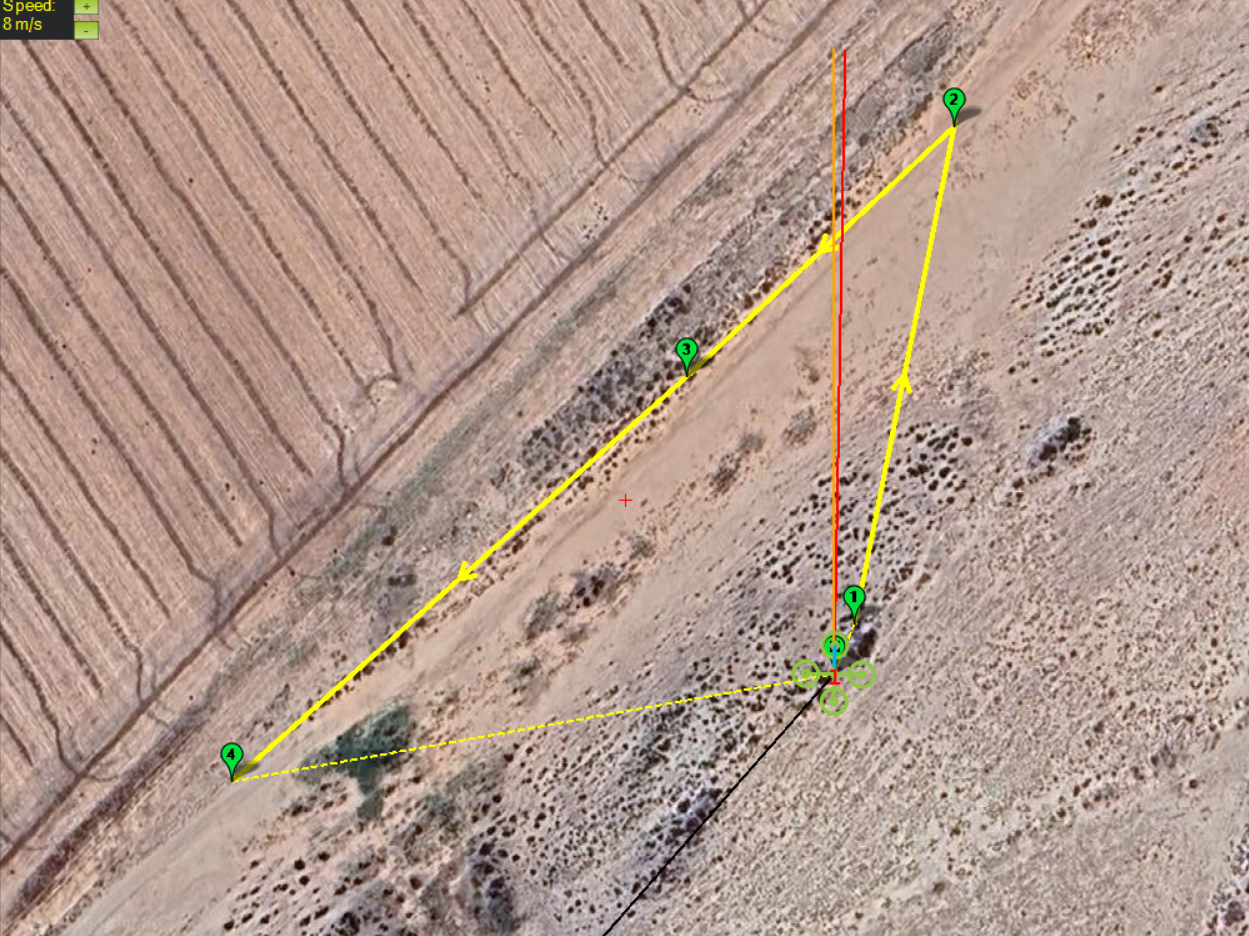
\includegraphics[width=0.47\textwidth]{Main/images/Nominal_trajectory_mission.png}}
\hfill
\subfloat[\centering]{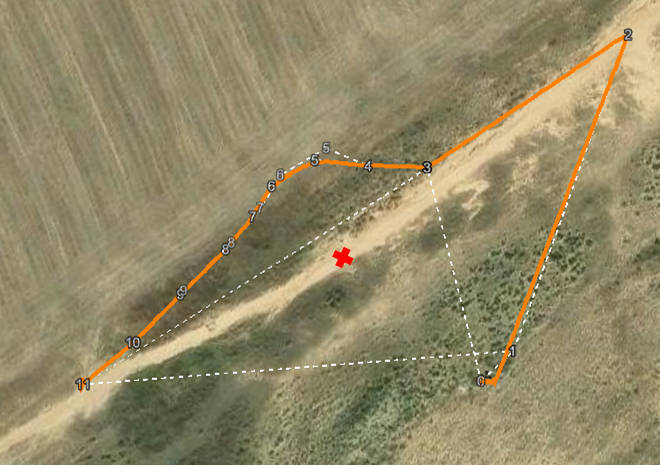
\includegraphics[width=0.47\textwidth]{Main/images/Log_route_replanning_x.png}}\\
\caption{\deleted{Real World Scenario Model Representation:}\added{Real-world trajectory comparison:} \textbf{(a)} nominal waypoint mission and \textbf{(b)} route reconstructed from the flight log.\label{fig:real_world_comparison}}
\end{figure}

\deleted{Finally, figure }\added{Figure~}\ref{fig:real_world_comparison} \deleted{represents on the left side}\added{compares} the nominal \deleted{waypoints Mission that is downloaded into the autopilot, and on the right side the final route reported in one of the performed flights, extracted}\added{waypoint mission with the route reconstructed from one physical-flight log. The obstacle location is marked in the visualization, and the executed track shows the deviation} from the \deleted{flight log given by the autopilot. From the comparison of those images it can be appreciated how the obstacles (represented as a red X in the images) appear in the camera FOV and,}\added{nominal corridor} after the \deleted{processing of the data by the YOLO by the onboard computer and detected that the }reaction \deleted{range}\added{condition} is reached, \deleted{the system has performed the avoiding maneuver, changing the nominal}\added{followed by the return toward the planned} route.

\deleted{After these evaluations of the logs, it can be concluded}\added{The field logs and trajectory comparison demonstrate that PORCE was integrated into the experimental UAS architecture, that obstacle-triggered local replanning was executed in flight, and} that the \deleted{system also works in a real world scenario mounted in an UAS architecture.}\added{vehicle subsequently returned toward the nominal mission trajectory.} \reviewnote{Aqu\'i nos siguen faltando las m\'etricas agregadas de la campa\~na real para pasar de ``lo vemos en el vuelo'' a una validaci\'on cuantitativa comparable con simulaci\'on.} 

\section{\added{Limitations}}

\added{The demonstrated operational envelope must be interpreted narrowly. The simulation campaign quantitatively documents dormancy, triggering, bounded bypass, and route reattachment for static protected regions represented by livestock. The field campaign demonstrates real-UAS integration and execution of the same avoidance logic, but the current manuscript does not yet report the same complete set of aggregate metrics for the real flights. The configured 12~m safety radius is an operational heuristic and has not yet been validated as a formal SORA-derived separation envelope. Clearance is evaluated relative to perceived obstacle positions; therefore, a direct ground-truth characterization of monocular geopositioning error remains necessary before the radius can be interpreted as a verified physical separation guarantee.}

\added{The local planner is two-dimensional and preserves the mission altitude; vertical avoidance and 3D obstacles intersecting the flight level are outside the present formulation. The landing segment is executed as part of the mission/autopilot logic and is not optimized by PORCE. The current results also do not establish comparative superiority over RRT*, DWA, ESLS, EAODA, or learning-based planners because those methods have not been reported under an identical experimental protocol in the supplied evidence. Likewise, systematic sensitivity analysis of the reaction-horizon and obstacle-inflation parameters, controlled robustness tests under perception/geopositioning errors, and representative onboard runtime/resource measurements remain necessary to close the corresponding reviewer requests quantitatively.}

\reviewnote{Nos siguen faltando estas piezas si no aparecen en datos adicionales: (1) sensibilidad de $R_s$, $D_{base}$, $k_v$ y velocidad; (2) accuracy de YOLO y error de geoposicionamiento contra ground truth; (3) benchmarks homog\'eneos frente a A*/RRT*/DWA y, si procede, ESLS/EAODA; (4) perturbaciones controladas de percepci\'on/posici\'onamiento; (5) escenarios con m\'ultiples obst\'aculos y objetivos din\'amicos si queremos reclamarlos dentro de este art\'iculo; (6) runtime, frecuencia efectiva y uso de recursos en hardware embarcado; y (7) m\'etricas completas y n\'umero de repeticiones de la campa\~na real. Si alguna de estas cosas ya est\'a en logs o v\'ideos, primero la extraemos; s\'olo repetimos experimentos cuando la evidencia no exista.}

\section{Conclusions}

This paper has presented PORCE, a deterministic local replanning method for waypoint-preserving obstacle avoidance in autonomous power-line inspection missions\deleted{, and has demonstrated it end-to-end inside a georeferenced Unreal Engine/Cesium simulation workflow. The central}\added{. Its} contribution is not \deleted{obstacle avoidance itself, which is a mature field}\added{a new detector or shortest-path algorithm}, but the integration of \deleted{the}\added{live georeferenced detections, temporary protected regions, speed-adaptive activation, bounded local replanning, failsafe escalation, and route reattachment within the running mission. This controller behavior is motivated by} European ground-risk \deleted{logic into the online controller: live detections are converted into protected local regions with hard safety radii, so the vehicle performs a conservative, auditable detour instead of overflying them, and the global inspection Mission resumes automatically once the conflict is resolved.}\added{and no-overflight considerations, while the present evidence deliberately stops short of claiming formal regulatory compliance.}

\deleted{In addition to its methodological contribution, the proposed guidance solution is relevant because it can be implemented, evaluated, and refined within a simulation environment prior to flight}\added{The simulation workflow provides a controlled environment for exercising the decision chain and extracting mission-level metrics before field} deployment. The \deleted{simulation framework makes it possible to reproduce different operational conditions in a controlled manner, analyze the response of the guidance system, and identify limitations before conducting real-flight tests. This is particularly relevant for industrial applications, where experimental campaigns involve considerable cost, time, and operational risk. The subsequent field tests presented in the results further support this development approach by demonstrating}\added{physical-flight evidence separately demonstrates} that the \deleted{proposed method}\added{same PORCE architecture} can be integrated \deleted{into the onboard UAS architecture and executed in a real-world scenario. Moreover, the comparison between simulation results and data obtained from real flights indicates that the simulated scenarios provide a representative basis for system development and pre-flight validation. The proposed workflow therefore supports not only the evaluation and refinement of the guidance solution in simulation, but also its progressive transfer and validation under real operating conditions, contributing to its maturation towards practical deployment.}\added{onboard and can execute an obstacle-triggered detour followed by route reattachment. Because the current field section does not yet report the same aggregate metrics as the simulation campaign, we do not infer quantitative simulation--flight equivalence or representativeness from these results. Establishing that relationship requires matched metrics and repeated runs in both environments.}

\deleted{In general, the results obtained in both simulation and real-world testing demonstrate that the proposed method is effective in addressing the operational challenges considered in this work.}\added{Within the demonstrated scope, the simulation evidence shows a first trigger at 60.1~m for a 61~m configured horizon, a minimum logged distance of 29.6~m to the nearest perceived obstacle in the audited run (20.6~m in the worst archived evasion run), evasion segments of approximately 28--35~s, and a path-length increase below 1\% for the complete evasion missions. The field evidence additionally demonstrates onboard integration, obstacle-triggered trajectory modification, and reattachment behavior in a physical UAS. These results support the feasibility of the controller architecture while the limitations above delimit the claims that can presently be made about regulatory compliance, physical clearance, perception accuracy, robustness, comparative performance, and real-time computational performance.}

\added{Future work will focus on the validation gaps identified above: quantitatively sizing class-dependent safety envelopes against perception/geopositioning uncertainty and the applicable ground-risk model; measuring runtime and resource use on representative onboard hardware; evaluating sensitivity to the reaction-horizon and inflation parameters; benchmarking the controller against representative local planners under the same mission protocol; and extending the demonstrated envelope to denser multi-obstacle, dynamic-obstacle, and uncertainty-aware scenarios. Multi-objective formulations that jointly account for path length, energy, mission completion time, and ground-risk exposure are also a natural extension of the present hard-constraint design.}


%%%%%%%%%%%%%%%%%%%%%%%%%%%%%%%%%%%%%%%%%%
%%%%%%%%%%%%%%%%%%%%%%%%%%%%%%%%%%%%%%%%%%
\vspace{6pt} 

%%%%%%%%%%%%%%%%%%%%%%%%%%%%%%%%%%%%%%%%%%
%% optional
%\supplementary{The following supporting information can be downloaded at \linksupplementary{s1}, Figure S1: title; Table S1: title; Video S1: title.}

% Only for journal Methods and Protocols:
% If you wish to submit a video article, please do so with any other supplementary material.
% \supplementary{The following supporting information can be downloaded at \linksupplementary{s1}, Figure S1: title; Table S1: title; Video S1: title. A supporting video article is available at doi: link.}

% Only used for preprtints:
% \supplementary{The following supporting information can be downloaded at the website of this paper posted on \href{https://www.preprints.org/}{Preprints.org}.}

% Only for journal Hardware:
% If you wish to submit a video article, please do so with any other supplementary material.
% \supplementary{The following supporting information can be downloaded at \linksupplementary{s1}, Figure S1: title; Table S1: title; Video S1: title.\vspace{6pt}\\
%\begin{tabularx}{\textwidth}{lll}
%\toprule
%\textbf{Name} & \textbf{Type} & \textbf{Description} \\
%\midrule
%S1 & Python script (.py) & Script of python source code used in XX \\
%S2 & Text (.txt) & Script of modelling code used to make Figure X \\
%S3 & Text (.txt) & Raw data from experiment X \\
%S4 & Video (.mp4) & Video demonstrating the hardware in use \\
%... & ... & ... \\
%\bottomrule
%\end{tabularx}
%}

%%%%%%%%%%%%%%%%%%%%%%%%%%%%%%%%%%%%%%%%%%
\supplementary{The following supporting information can be downloaded at \href{https://github.com/PabloPorce/PORCE-regulatory-compliant-static-obstacle-avoidance-solution-for-UAS-for-Powerline-Inspection/tree/main}{Video S1}: annotated perception output of the cattle-evasion encounter, recorded from the onboard camera of the simulated UAS with the detection and tracking overlays produced by the vision front-end.}

\authorcontributions{Conceptualization, P.D.P. and J.V.; methodology, P.D.P., X.O. and D.A.; software, P.D.P, X.O. and D.A.; validation, X.O. and D.A.; formal analysis, P.D.P. and J.V.; investigation, P.D.P. and X.O.; resources, P.D.P. and J.V.; data curation, X.O.; writing---original draft preparation, P.D.P. and X.O.; writing---review and editing, J.V. and D.A.; visualization, X.O.; supervision, J.V.; project administration, J.V. All authors have read and agreed to the published version of the manuscript.}

\funding{This work was supported by the project \textit{Entornos Cognitivos para el Envejecimiento Aut\'onomo, Activo y Saludable} [grant number PID2024-158490OB-C32]; the project ElectroDron [grant number CPP2024-011509]; the project H2DRON [grant number 0011-1411-2024-000038]; and the project FREEDRONE [grant number 0011-1411-2025-000086]}

\institutionalreview{Not applicable.}

\informedconsent{Not applicable.}

\dataavailability{The code, \deleted{Mission}\added{mission} files, simulation defaults, and run archives (telemetry streams and decision logs) supporting the reported results are available \deleted{under}\added{from the authors upon} consultation\deleted{ due to}\added{, subject to the applicable} privacy \deleted{reasons.}\added{constraints.} The annotated encounter video is provided as Supplementary Video S1.}

%\durcstatement{Current research is limited to the [please insert a specific academic field, e.g., XXX], which is beneficial [share benefits and/or primary use] and does not pose a threat to public health or national security. Authors acknowledge the dual-use potential of the research involving xxx and confirm that all necessary precautions have been taken to prevent potential misuse. As an ethical responsibility, authors strictly adhere to relevant national and international laws about DURC. Authors advocate for responsible deployment, ethical considerations, regulatory compliance, and transparent reporting to mitigate misuse risks and foster beneficial outcomes.}

% Only for journal Nursing Reports
%\publicinvolvement{Please describe how the public (patients, consumers, carers) were involved in the research. Consider reporting against the GRIPP2 (Guidance for Reporting Involvement of Patients and the Public) checklist. If the public were not involved in any aspect of the research add: ``No public involvement in any aspect of this research''.}
%
%% Only for journal Nursing Reports
%\guidelinesstandards{Please add a statement indicating which reporting guideline was used when drafting the report. For example, ``This manuscript was drafted against the XXX (the full name of reporting guidelines and citation) for XXX (type of research) research''. A complete list of reporting guidelines can be accessed via the equator network: \url{https://www.equator-network.org/}.}
%
%% Only for journal Nursing Reports
%\useofartificialintelligence{Please describe in detail any and all uses of artificial intelligence (AI) or AI-assisted tools used in the preparation of the manuscript. This may include, but is not limited to, language translation, language editing and grammar, or generating text. Alternatively, please state that “AI or AI-assisted tools were not used in drafting any aspect of this manuscript”.}

\acknowledgments{The authors thank the flight-operations team at FuVeX Civil SL for the operational feedback that motivated the inspection scenarios}

\conflictsofinterest{Pablo de Porcellinis is affiliated with FuVeX Civil SL. The remaining authors declare no conflicts of interest.}


%%%%%%%%%%%%%%%%%%%%%%%%%%%%%%%%%%%%%%%%%%
%% Optional

%% Only for journal Encyclopedia
%\entrylink{The Link to this entry published on the encyclopedia platform.}

\abbreviations{Abbreviations}{%
The following abbreviations are used in this manuscript:\\

\noindent 
\begin{tabular}{@{}ll}
A* & A-star graph search algorithm\\
AGL & Above Ground Level\\
AMC/GM & Acceptable Means of Compliance and Guidance Material\\
EASA & European Union Aviation Safety Agency\\
GNSS & Global Navigation Satellite Systems\\
JARUS & Joint Authorities for Rulemaking on Unmanned Systems\\
LTE & Long-Term Evolution\\
MSL & Mean Sea Level\\
OSO & Operational Safety Objective\\
PORCE & Path-Planning for Obstacle-Avoidance with Regulatory-Compliant Evasion\\
RTL & Return-to-Launch\\
SITL & Software-in-the-Loop\\
SORA & Specific Operations Risk Assessment\\
UAS & Unmanned Aircraft System\\
UAV & Unmanned Aerial Vehicle\\
WP & Waypoint\\
YOLO & You Only Look Once
\end{tabular}
}
\reviewnote{El acr\'onimo PORCE sigue expandi\'endose como ``Regulatory-Compliant Evasion'' porque as\'i se llama el m\'etodo original. Hemos quitado el claim de cumplimiento del t\'itulo y del texto cient\'ifico, pero si queremos eliminar por completo la ambig\"uedad del revisor tenemos que decidir si renombramos tambi\'en la expansi\'on del acr\'onimo o si dejamos claro en la respuesta que es un nombre hist\'orico y no una afirmaci\'on de aprobaci\'on regulatoria.}

\reftitle{References}
\bibliography{Main/references_main}
\end{document}

